\chapter{Protocolo de Experimentação para seleção de Métodos Matemáticos}

Esta seção descreve como foi percorrido o Protocolo de Experimentação para selecionar os Métodos Matemáticos que serão implementados na ferramenta InvestMVC. O Protocolo de Experimentação utilizado é uma adaptação do protocolo presente no Anexo A - Template de Protocolo Experimental.

Ao final do capítulo, o leitor será capaz de entender porque foi escolhido os métodos de Correlação de Pearson, Fibonacci e Mínimos Quadrados para serem incorporados na ferramenta InvestMVC.

\section{Preparação para o Protocolo}

A seguinte questão de pesquisa foi definida na capítulo 1: é possível desenvolver uma ferramenta multiparadigma que substitua os Experts convencionais do Mercado de Moedas? 

É necessário que a ferramenta InvestMVC tenha métodos relevantes para operar no Mercado de Moedas. Logo, é deve-se selecionar os métodos para serem implementados na ferramenta através de critérios bem definidos. A seleção dos métodos, critérios para realização dos experimentos, bem como resultados serão apresentados nas seções posteriores.

\section{Controle de Versão do Protocolo}

O controle de versão do protocolo desse experimento encontra-se no github\footnote{\url{https://github.com/cleitoncsg/investMVC}} da ferramenta InvestMVC.

\section{Projeto do Protocolo de Experimentação}

Nesta seção é definido as variáveis dependentes e independentes, critérios para seleção dos Métodos Matemáticos e definições para simulações dos métodos.


\subsection{Variáveis dependentes e independentes}
Variáveis independentes são aquelas que são manipuladas e as que variáveis dependentes são apenas medidas ou registradas. Os termos variável dependente e independente aplicam-se principalmente à pesquisa experimental, onde algumas variáveis são manipuladas \cite[pág.~13]{hoppen2010}.

Para se selecionar os métodos de operação no Mercado de Moedas da ferramenta InvestMVC, foi definido as seguintes variáveis independentes e seus respectivos valores a serem manipulados:

\begin{itemize}
\item Alavancagem com valor de 0.25;
\item Conta de simulação com valor inicial de 3.000 USD;
\item Margem de negociação/alavancagem da conta igual a 1:500;
\item Stop loss e take profit definido em 500 pontos.
\end{itemize}

Também foi definido as variáveis dependentes:

\begin{itemize}
\item Experts programados em linguagem MQL4;
\item Simulação realizada no mesmo período de tempo (agosto de 2012 à agosto de 2014);
\item Simulações realizadas na mesma máquina e mesmo sistema operacional.

\end{itemize}

\subsection{Critério para seleção dos Métodos Matemáticos}

Os Métodos Matemáticos implementados em linguagem MQL4 que obter lucro de 10\% do capital inicial serão aprovados no experimento.

\subsection{Definições para simulação dos métodos de operação}

Foi utilizado o simulador da plataforma Metatrader \footnote{\url{http://www.metatrader4.com/}} para realizar a simulação e, posteriormente, analisar os resultados e definir os métodos a serem implementados na ferramenta InvestMVC.

Através do simulador da plataforma Metatrader4, obteve-se o desempenho do expert CorrelacaoPearson.mql, MediaMovel.mql, MinimosQuadrados.mql, Estocastico.mql e Fibonacci.mql durante o período de agosto de 2012-2014.

\section{Execução e Análise dos dados}

Nesta seção é evidenciado os resultados  das simulações dos Experts em linguagem MQL4 (produto da implementação dos Métodos Matemáticos) através de relatórios e gráficos.

\subsection{Implementação dos Métodos Matemáticos}

Os métodos de Correlação Linear, Média Móvel, Mínimos Quadrados, Estocástico e Fibonacci foram implementados em linguagem MQL4 e assim foi construído um expert para cada método. Esses produtos de software receberam os nomes, respectivamente, CorrelacaoPearson.mql, MediaMovel.mql, MinimosQuadrados.mql, Estocastico.mql e Fibonacci.mql. Cada expert encontra-se no apêndice Métodos Matemáticos implementados em mql.

\subsection{Simulação do método de Correlação Linear}

O expert CorrelacaoPearson.mql obteve o percentual de negociações com lucros de 56.86\% no período agosto 2012-2013. Nesse período, o expert teve um lucro de 1981.60 USD.
 No período de agosto 2013-2014, o percentual de negociações com lucros foi de 55.56\%  e obteve-se o lucro de 1119.05 USD. 
Os relatórios completos das simulações podem ser visualizados nas figuras \ref{protocoloCorrelacao} e \ref{protocoloCorrelacao2}.

\begin{figure}[htp]
\centering
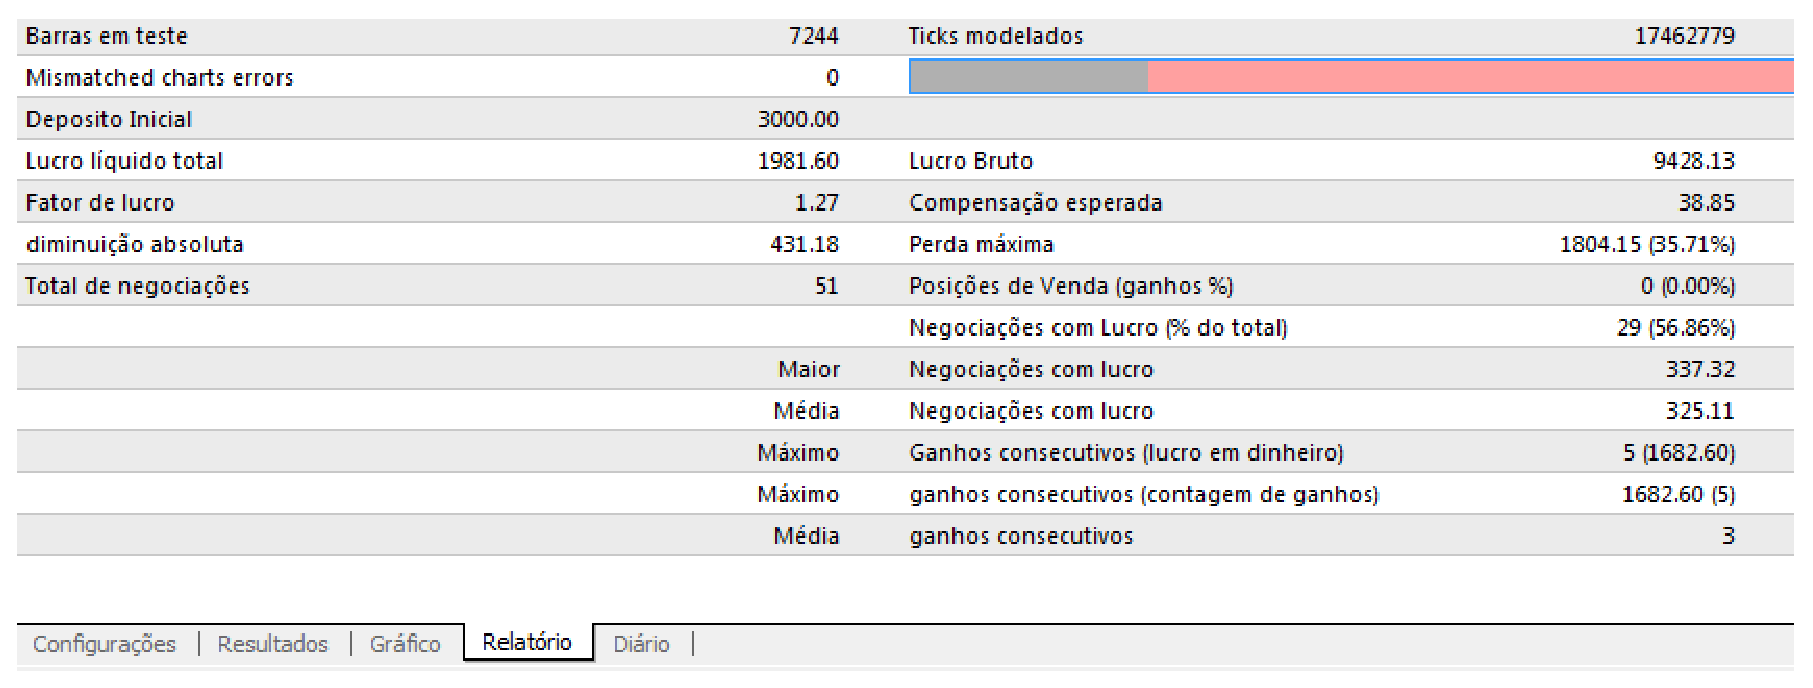
\includegraphics[width=0.9\textwidth]{figuras/protocoloCorrelacao}
\caption{Relatório de simulação no período agosto 2012-2013 do expert CorrelacaoPearson.mql}{Fonte: Autores} 
\label{protocoloCorrelacao}
\end{figure}

\begin{figure}[htp]
\centering

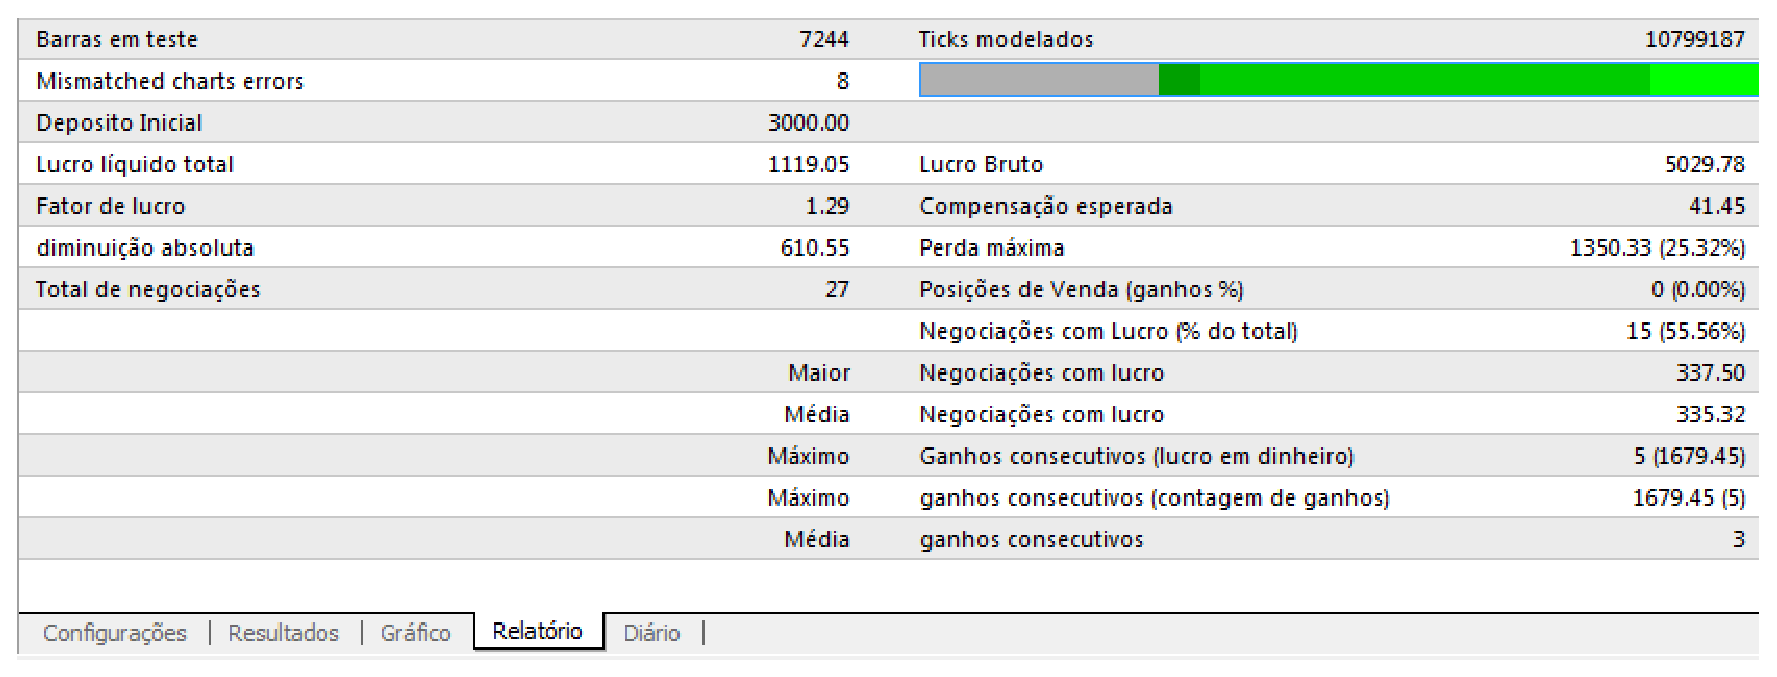
\includegraphics[width=0.9\textwidth]{figuras/protocoloCorrelacao2}
\caption{Relatório de simulação no período agosto 2013-2014 do expert CorrelacaoPearson.mql}{Fonte: Autores} 
\label{protocoloCorrelacao2}
\end{figure}

Foram gerados os gráficos de simulação 2012-2013 e 2013-2014. É possível perceber que o método de Correlação de Pearson, perde dinheiro em alguns períodos, mas os ganhos são superiores as perdas.

\begin{figure}[htp]
\centering
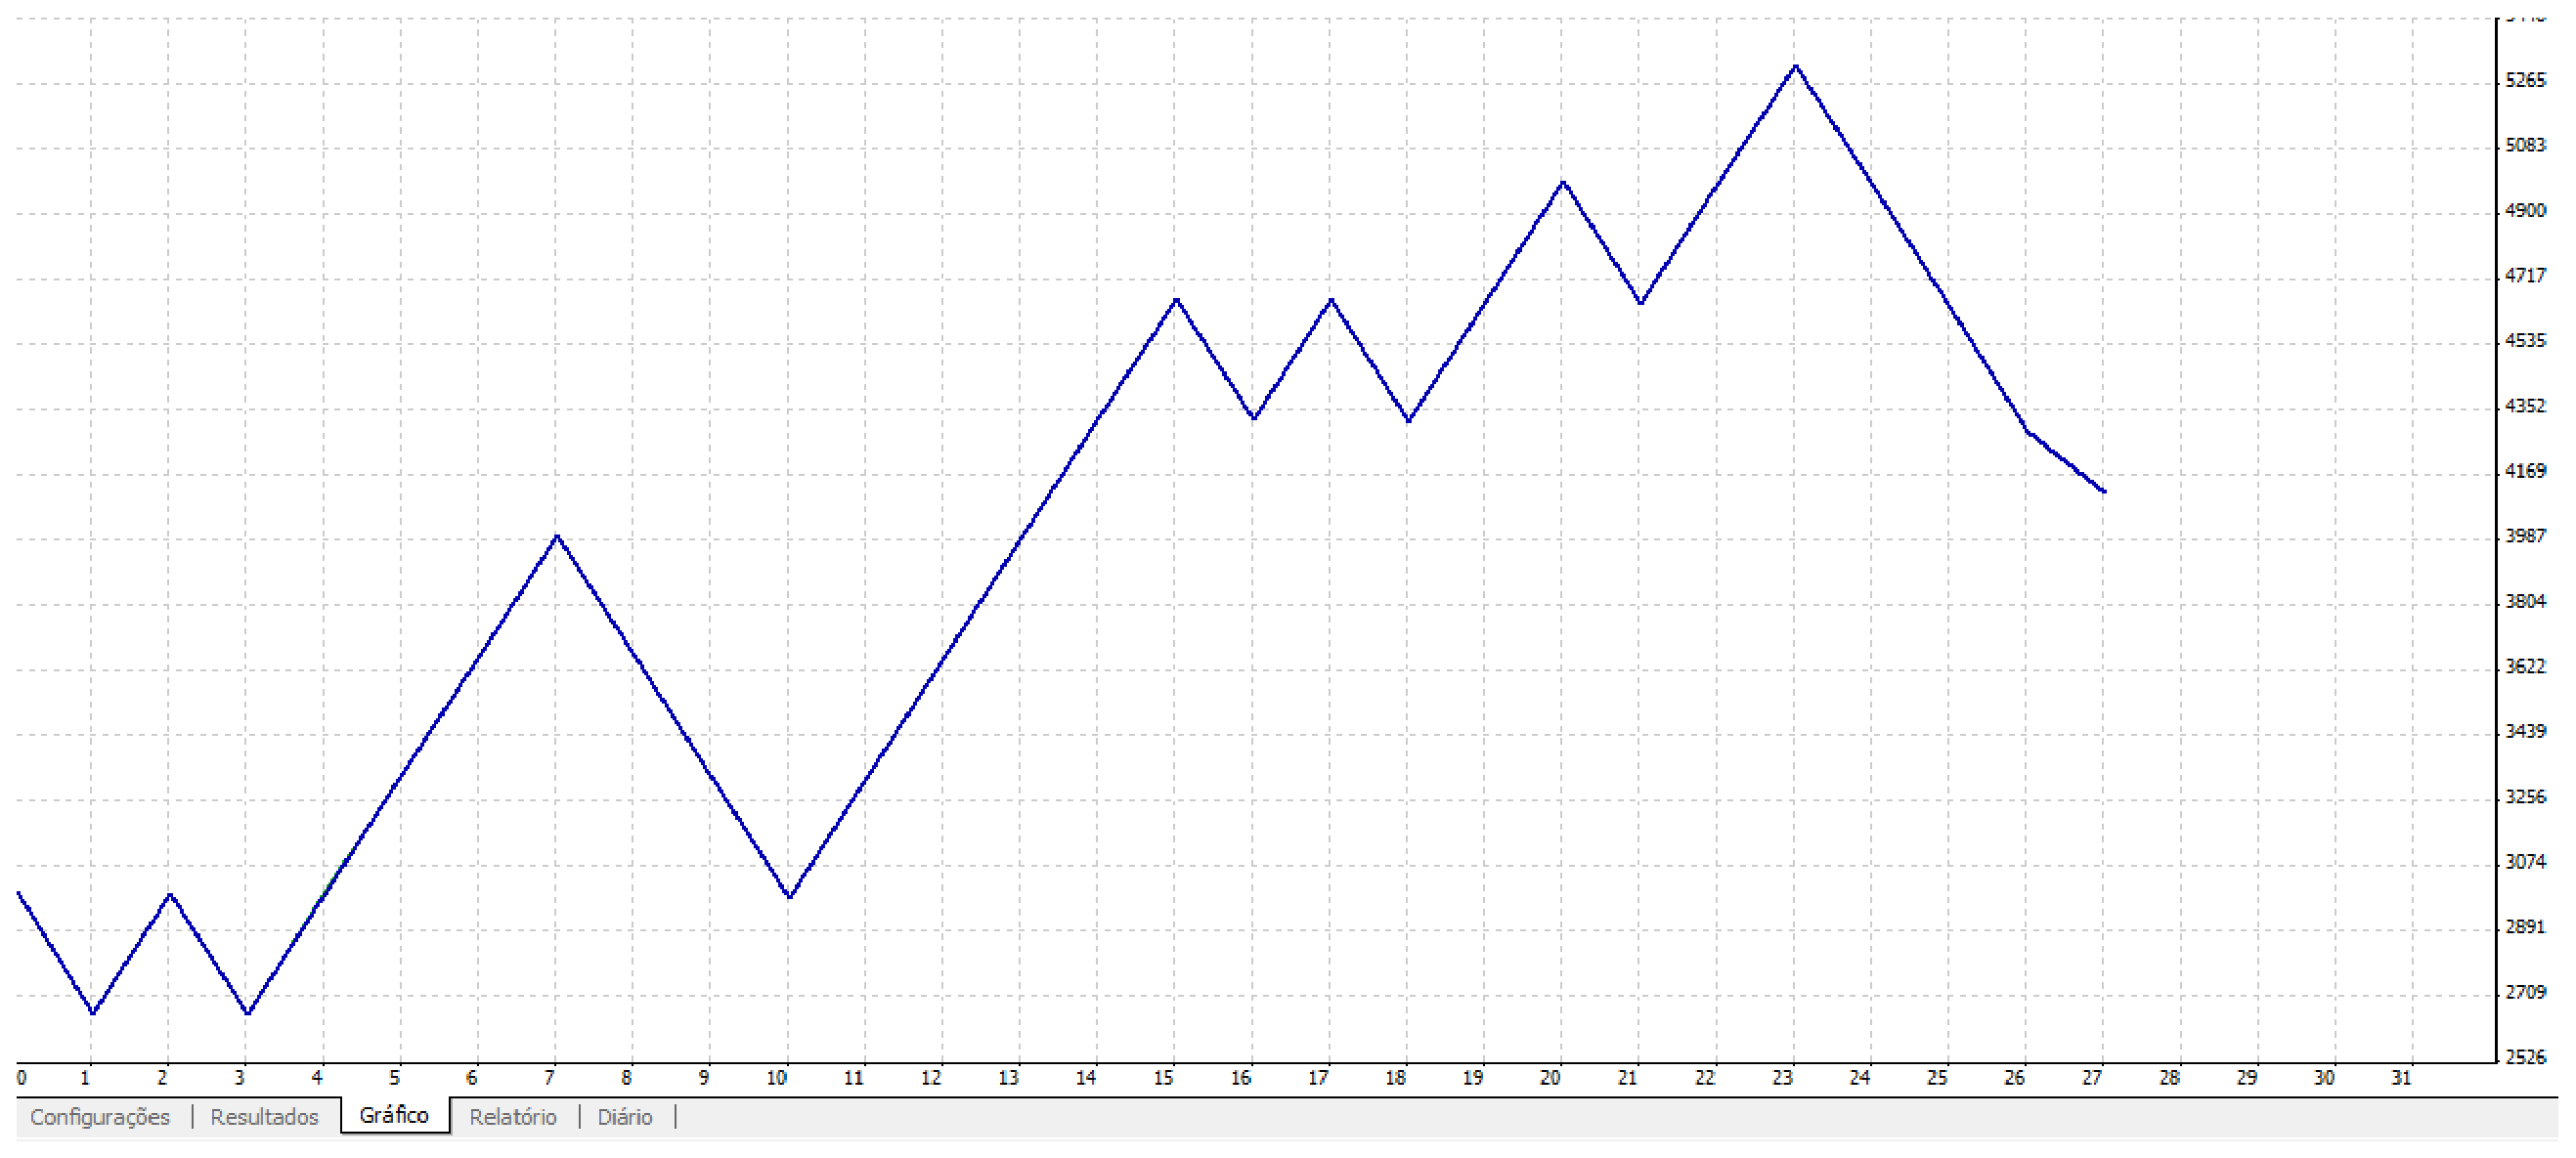
\includegraphics[width=0.9\textwidth]{figuras/protocoloCorrelacao3}
\caption{Gráfico gerado pela simulação do expert CorrelacaoPearson.mql no período agosto 2012-2013}{Fonte: Autores} 
\label{protocoloCorrelacao3}
\end{figure}

\begin{figure}[htp]
\centering
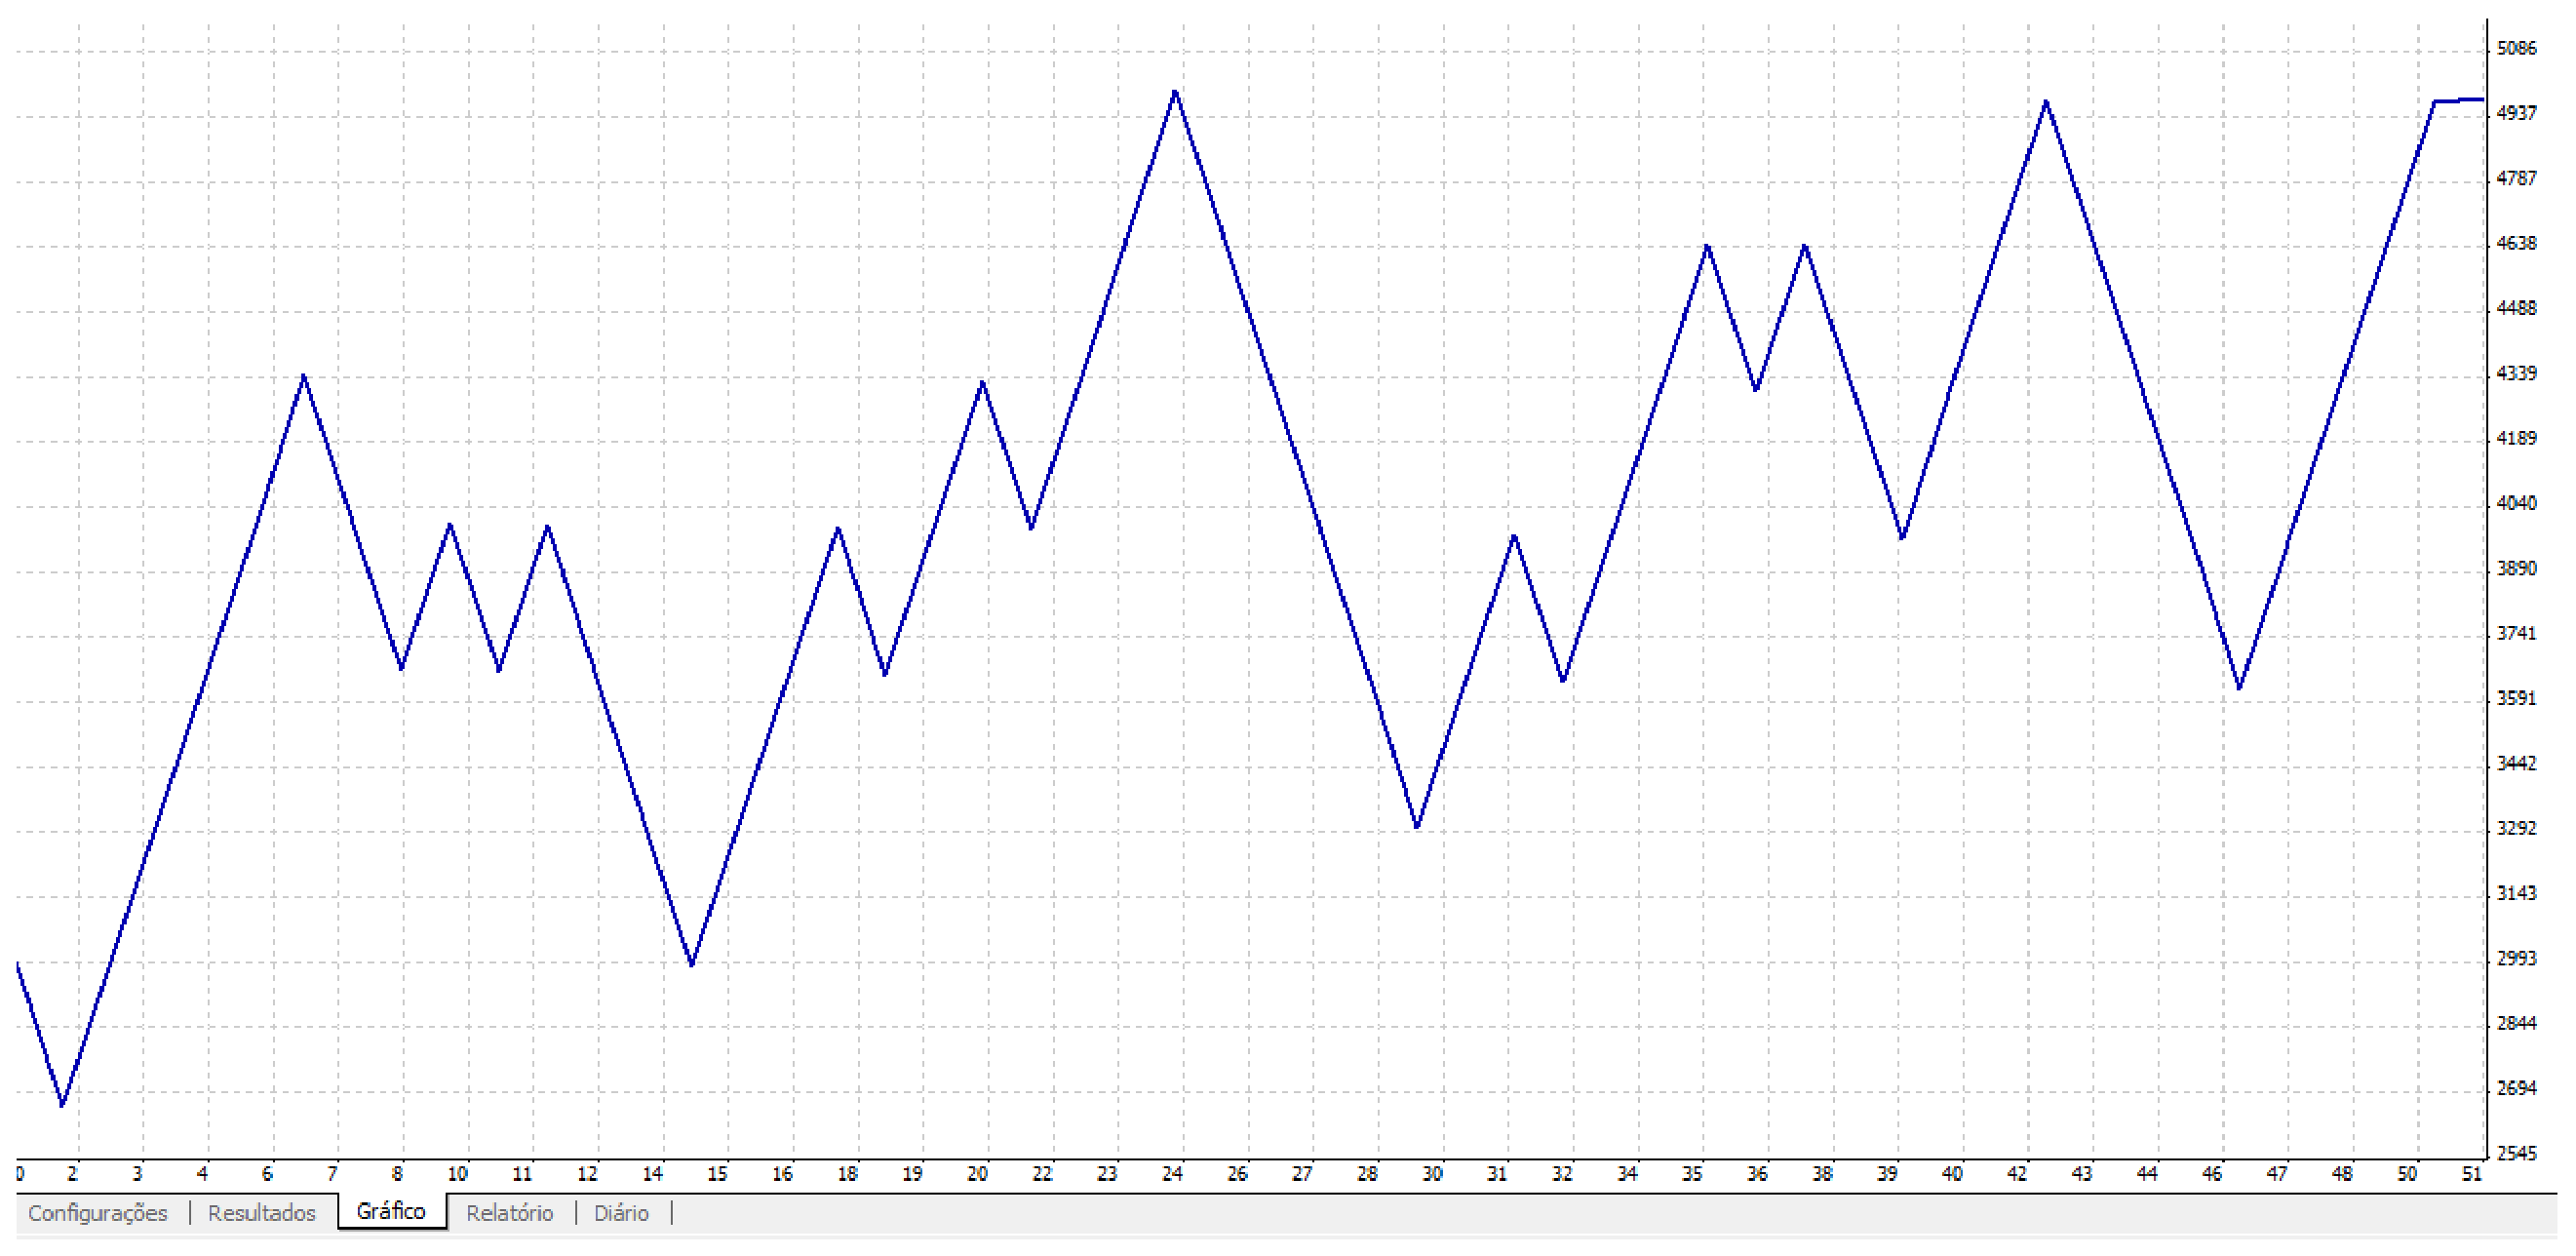
\includegraphics[width=0.9\textwidth]{figuras/protocoloCorrelacao4}
\caption{Gráfico gerado pela simulação do expert CorrelacaoPearson.mql no período agosto 2013-2014}{Fonte: Autores} 
\label{protocoloCorrelacao4}
\end{figure}

\subsection{Simulação do método de Mínimos Quadrados}

O expert MinimosQuadrados.mql obteve o percentual de negociações com lucros de 77.88\% no período agosto 2012-2013 e o  lucro nesse período foi de 1341.88 USD.
 No período de agosto 2013-2014, o percentual de negociações com lucros foi de 85.71\%  e obteve-se o lucro de 1026 USD. 
Os relatórios completos das simulações podem ser visualizados nas figuras \ref{protocoloMinimos} e \ref{protocoloMinimos2}.

\begin{figure}[htp]
\centering
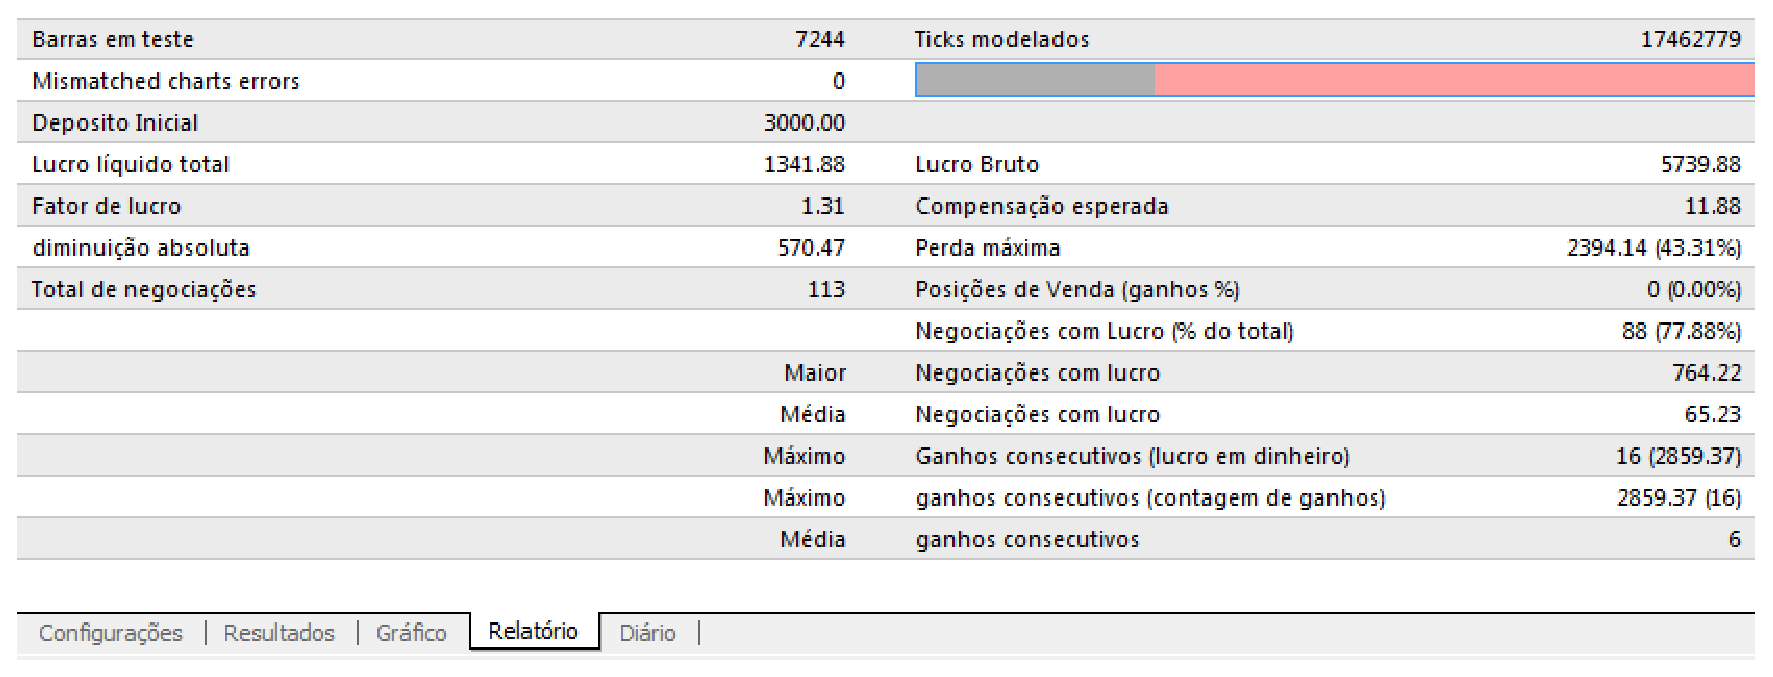
\includegraphics[width=0.9\textwidth]{figuras/protocoloMinimos}
\caption{Relatório de simulação no período agosto 2012-2013 do expert}{Fonte: Autores} 
\label{protocoloMinimos}
\end{figure}

\begin{figure}[htp]
\centering
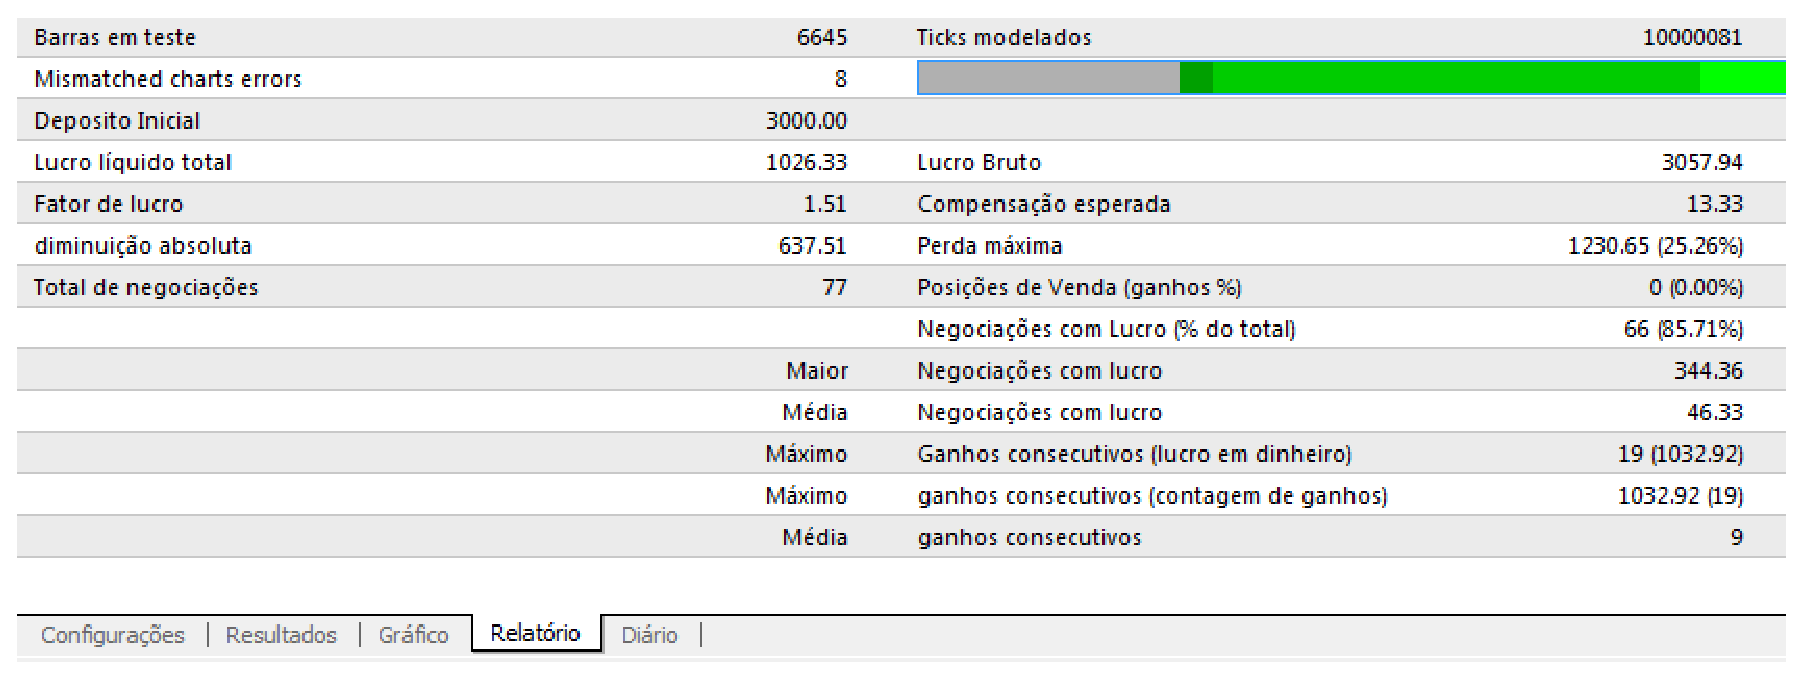
\includegraphics[width=0.9\textwidth]{figuras/protocoloMinimos2}
\caption{Relatório de simulação no período agosto 2012-2013 do expert}{Fonte: Autores} 
\label{protocoloMinimos2}
\end{figure}

O expert MinimosQuadrados.mql, teve altos e baixos nas simulações durante os dois anos (2012-2013 e 2013-2014). Mas, no desempenho geral, conforme é evidenciado nos gráficos, o expert teve um desempenho satisfatório.

\begin{figure}[htp]
\centering
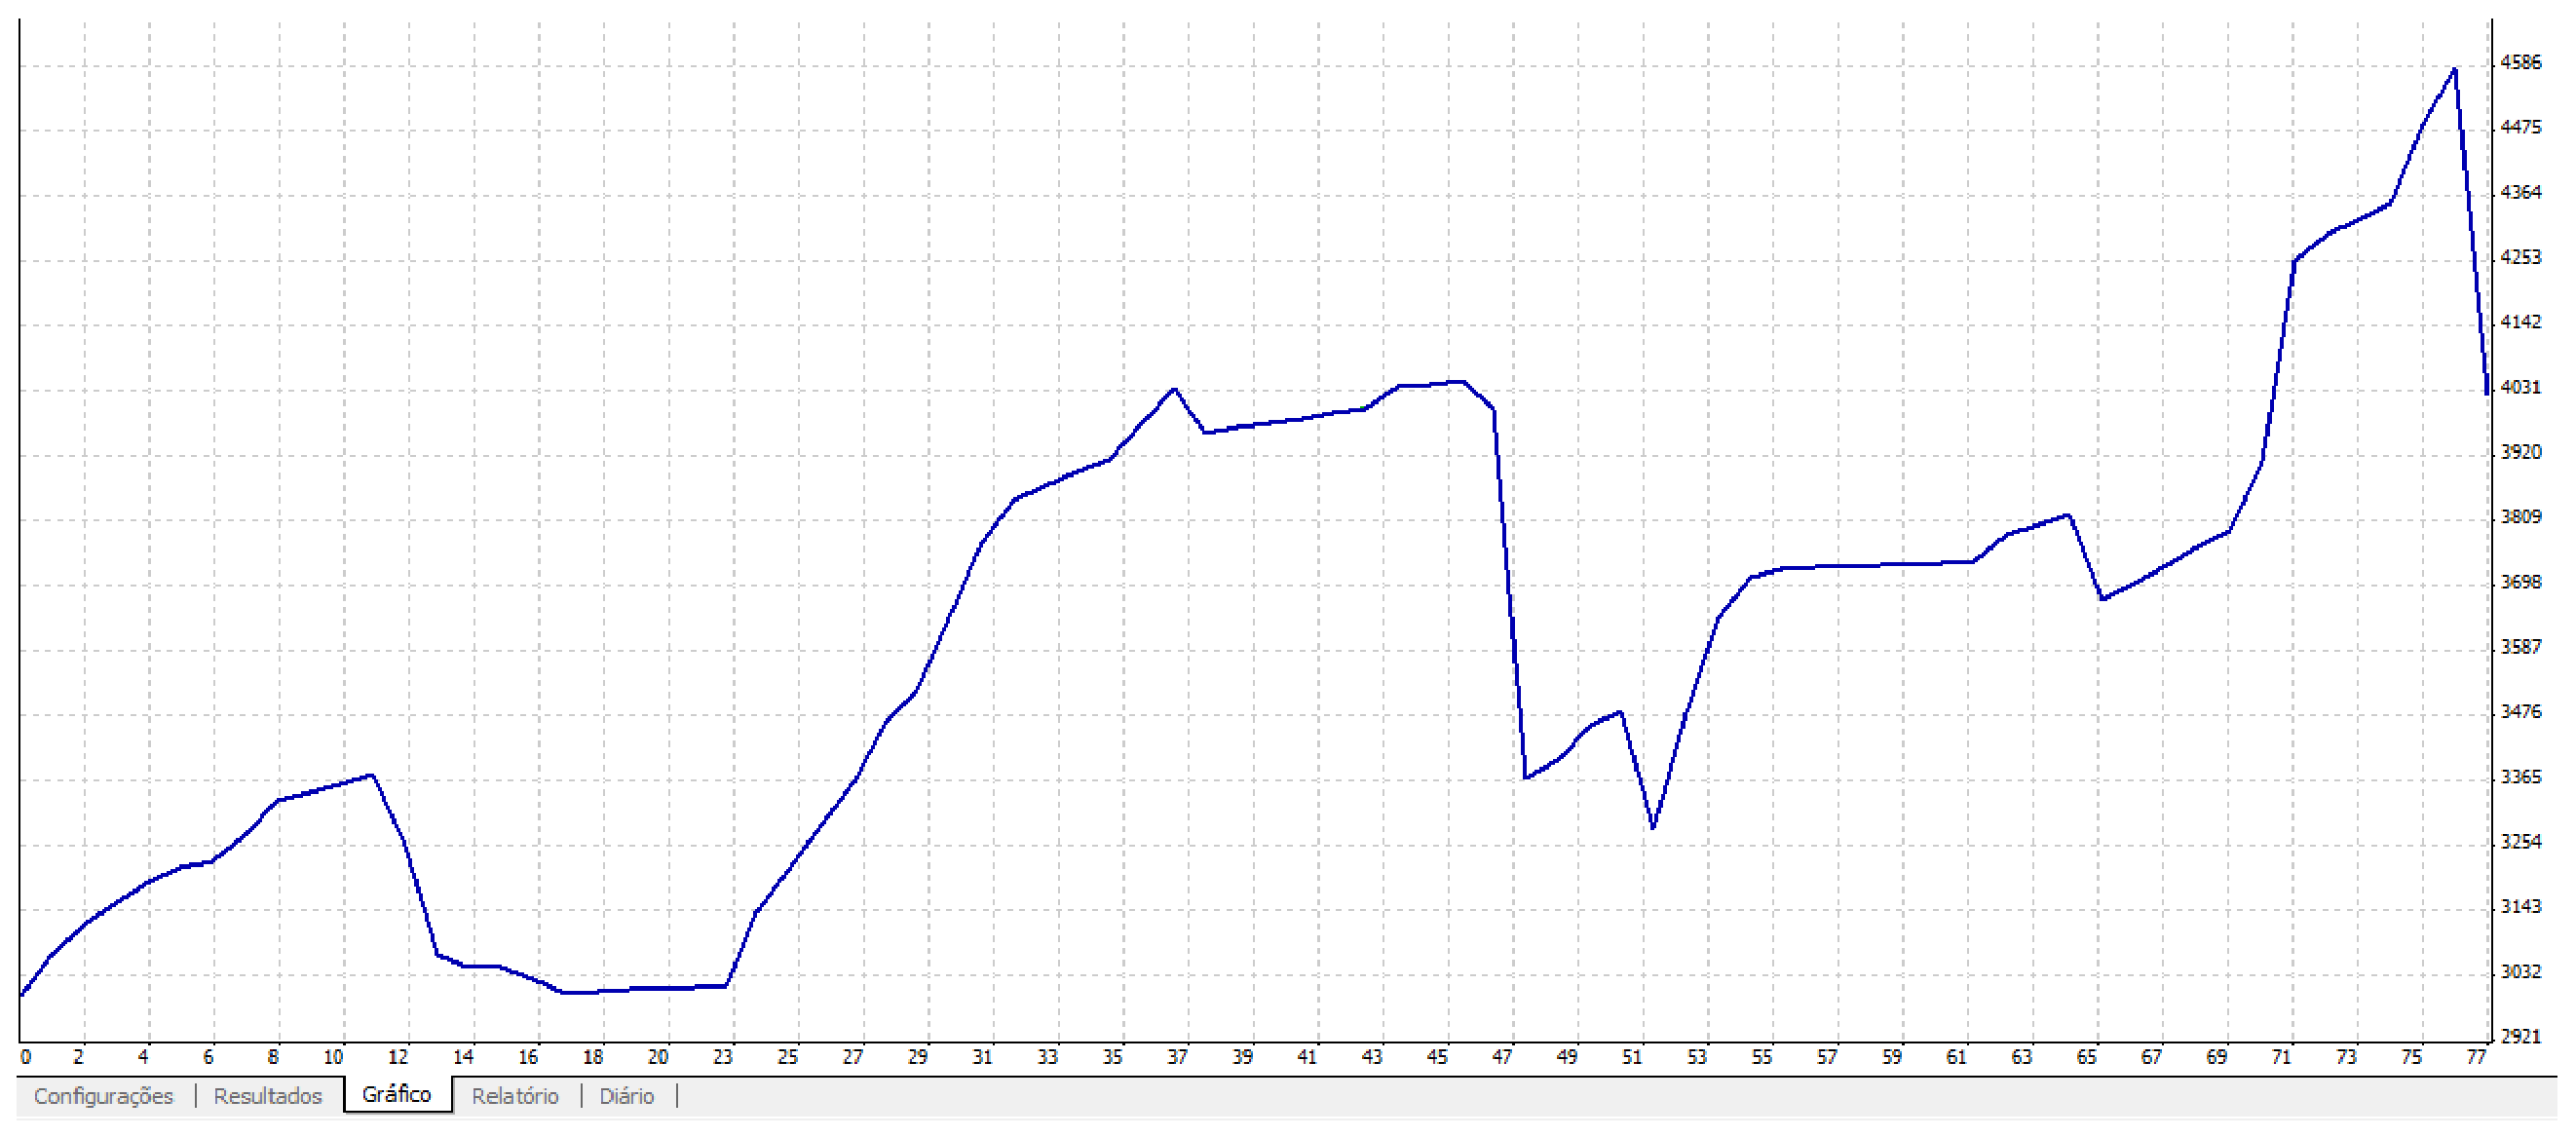
\includegraphics[width=0.9\textwidth]{figuras/protocoloMinimos3}
\caption{Relatório de simulação no período agosto 2012-2013 do expert}{Fonte: Autores} 
\label{protocoloMinimos3}
\end{figure}

\begin{figure}[htp]
\centering
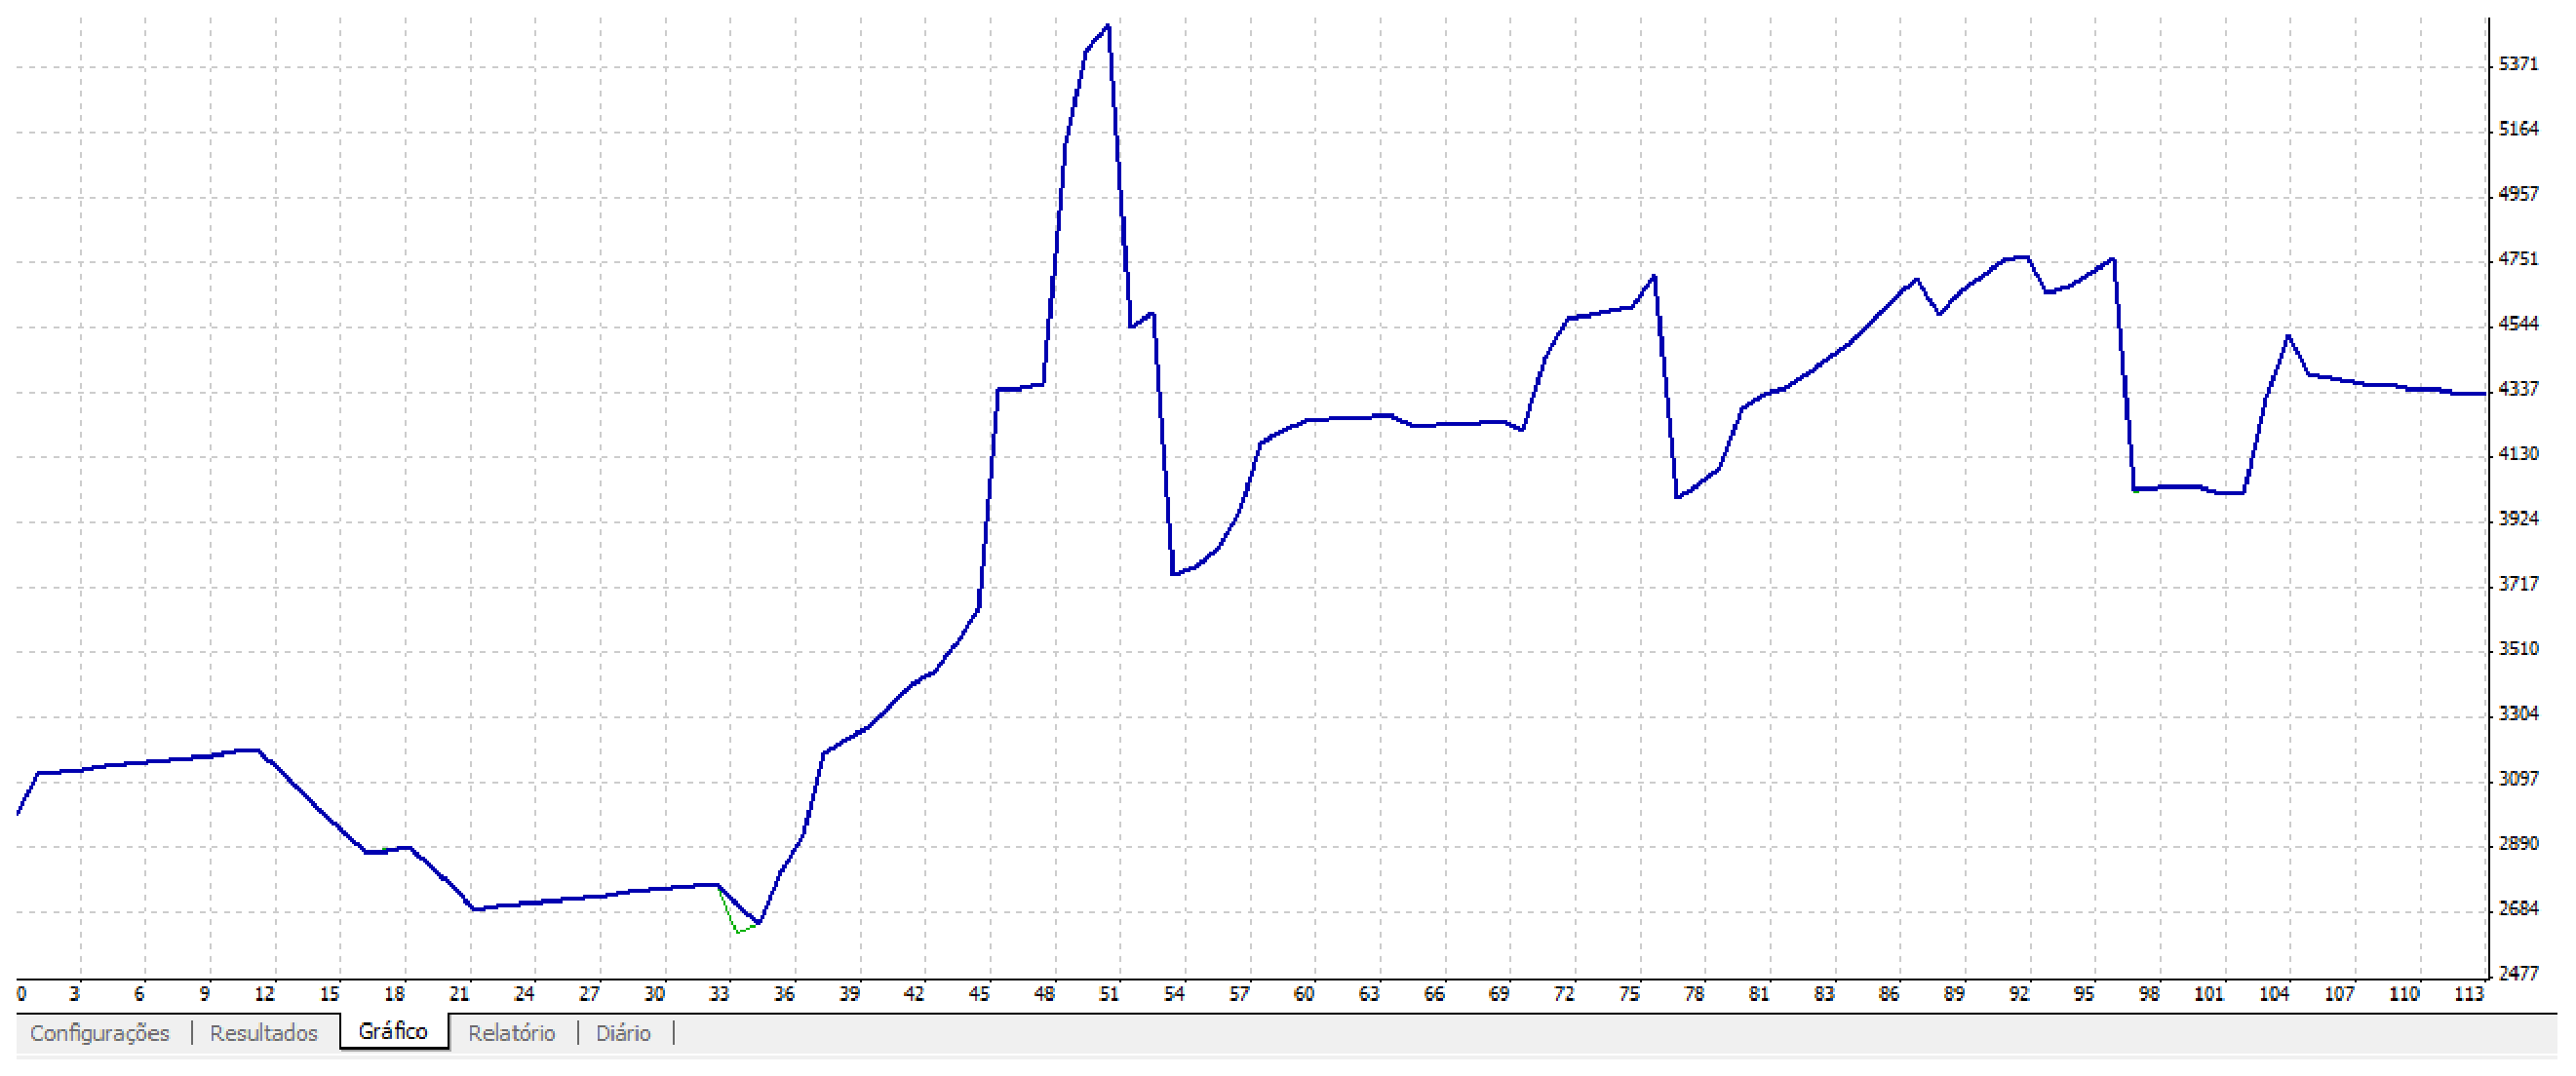
\includegraphics[width=0.9\textwidth]{figuras/protocoloMinimos4}
\caption{Relatório de simulação no período agosto 2013-2014 do expert}{Fonte: Autores} 
\label{protocoloMinimos4}
\end{figure}

\subsection{Simulação do método de Fibonacci}

O expert Fibonacci.mql obteve o percentual de negociações com lucros de 72.73\% no período agosto 2012-2013 e o  lucro nesse período foi de 341.20 USD.
No período de agosto 2013-2014, o percentual de negociações com lucros foi de 56.00\%  e obteve-se o lucro de 659.05 USD. Apesar do percentual de acerto nesse período ter sido menor quando comparado ao período de agosto 2012-2013, o lucro obtido foi 51.77\% maior. Isso se deve ao fato de no período de agosto 2013-2014, o expert ter negociado mais vezes (25 contra 11).

Os relatórios completos das simulações podem ser visualizados nas figuras \ref{protocoloFib} e \ref{protocoloFib2}.

\begin{figure}[htp]
\centering
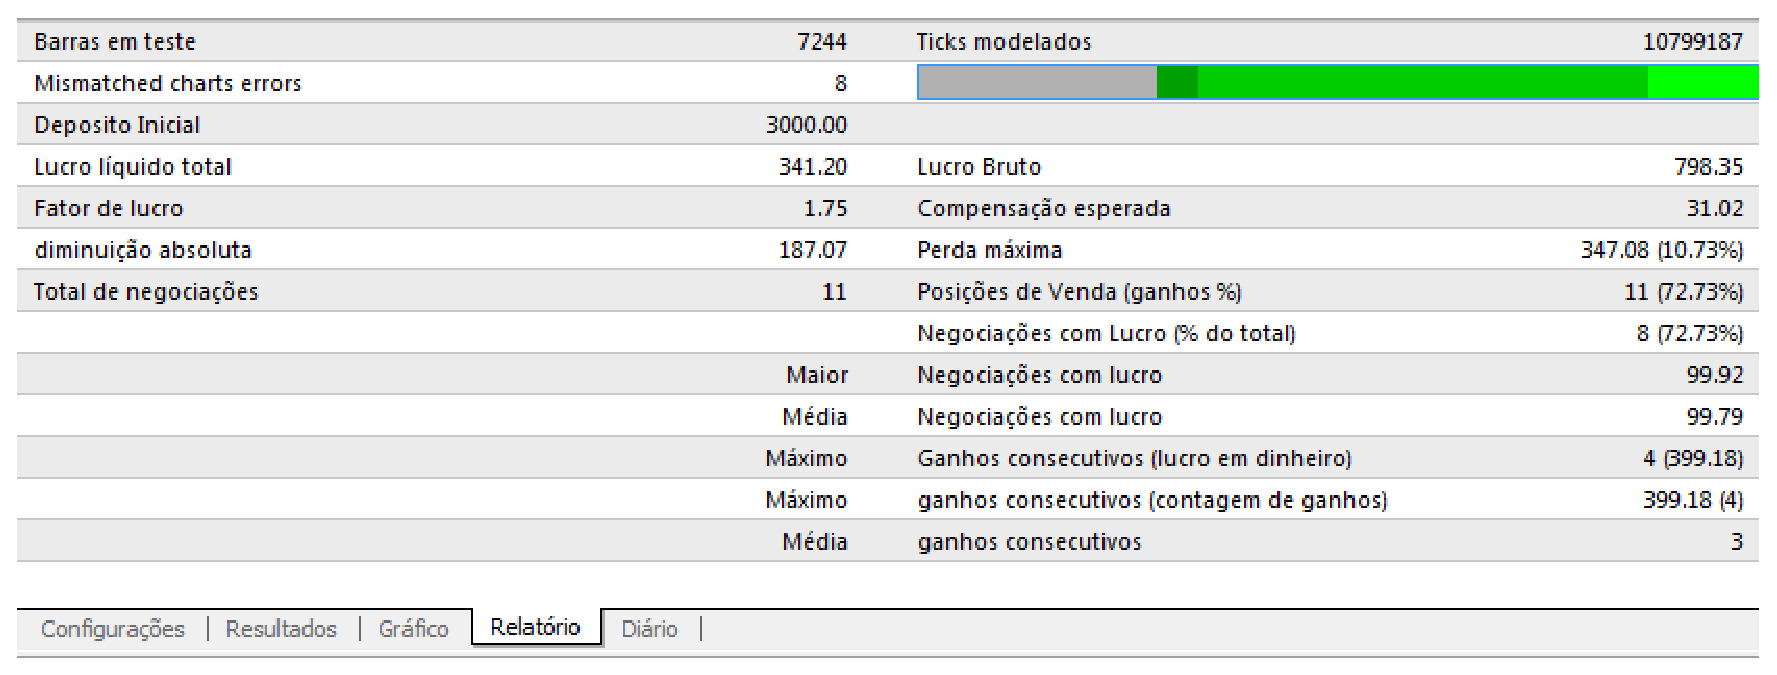
\includegraphics[width=0.9\textwidth]{figuras/protocoloFib}
\caption{Relatório de simulação no período agosto 2012-2013 do expert}{Fonte: Autores} 
\label{protocoloFib}
\end{figure}

\begin{figure}[htp]
\centering
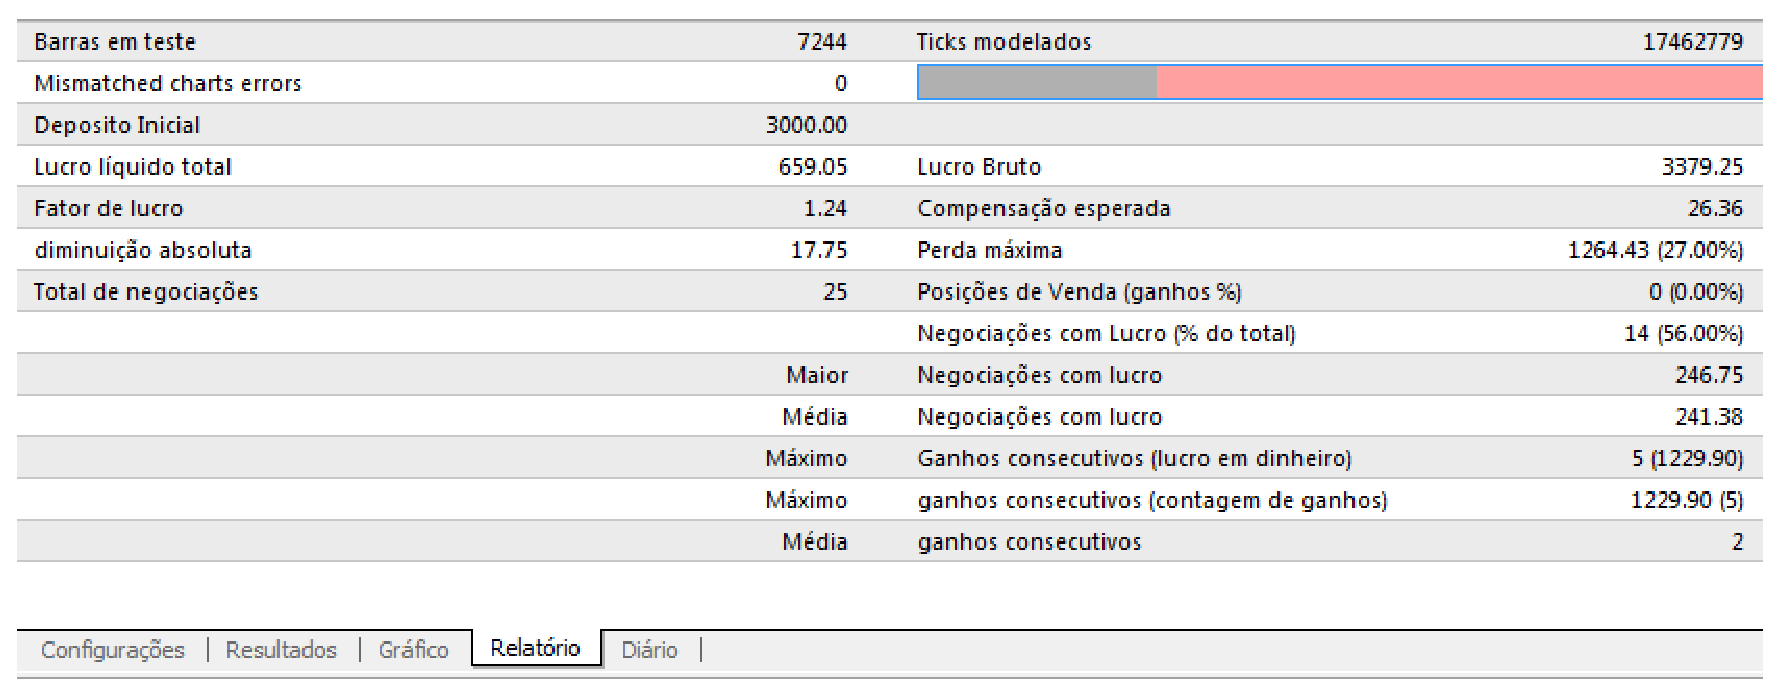
\includegraphics[width=0.9\textwidth]{figuras/protocoloFib2}
\caption{Relatório de simulação no período agosto 2013-2014 do expert}{Fonte: Autores} 
\label{protocoloFib2}
\end{figure}

É possível visualizar nos gráficos das simulações, as perdas de capital que o expert Fibonacci.mql gerou.

\begin{figure}[htp]
\centering
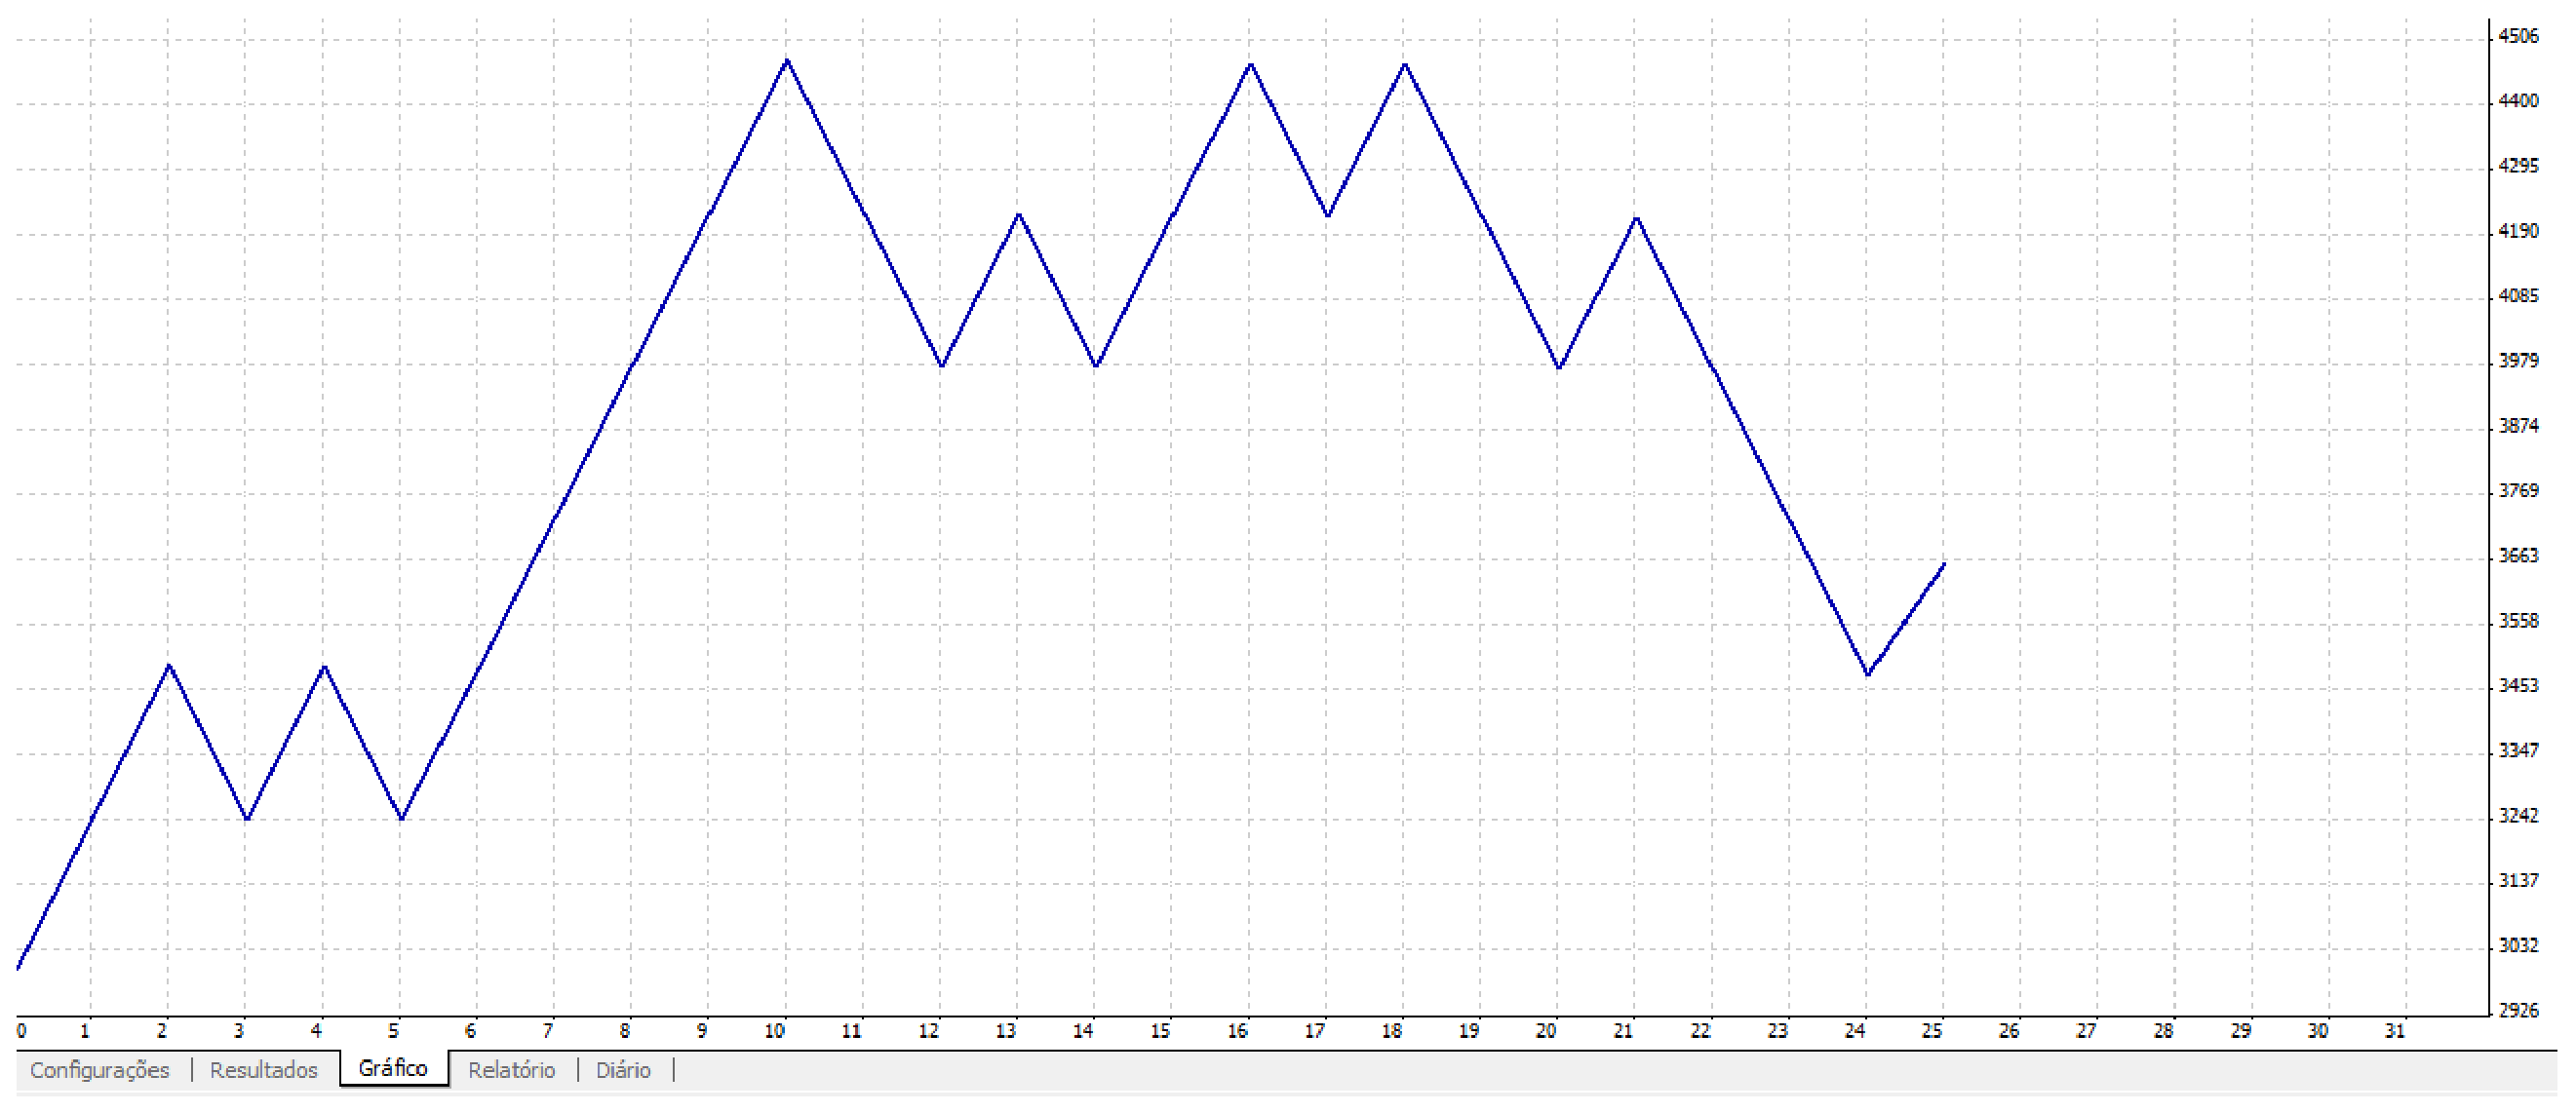
\includegraphics[width=0.9\textwidth]{figuras/protocoloFib3}
\caption{Gráfico gerado pela simulação do expert Fibonacci.mql no período agosto 2012-2013}{Fonte: Autores} 
\label{protocoloFib3}
\end{figure}

\begin{figure}[htp]
\centering
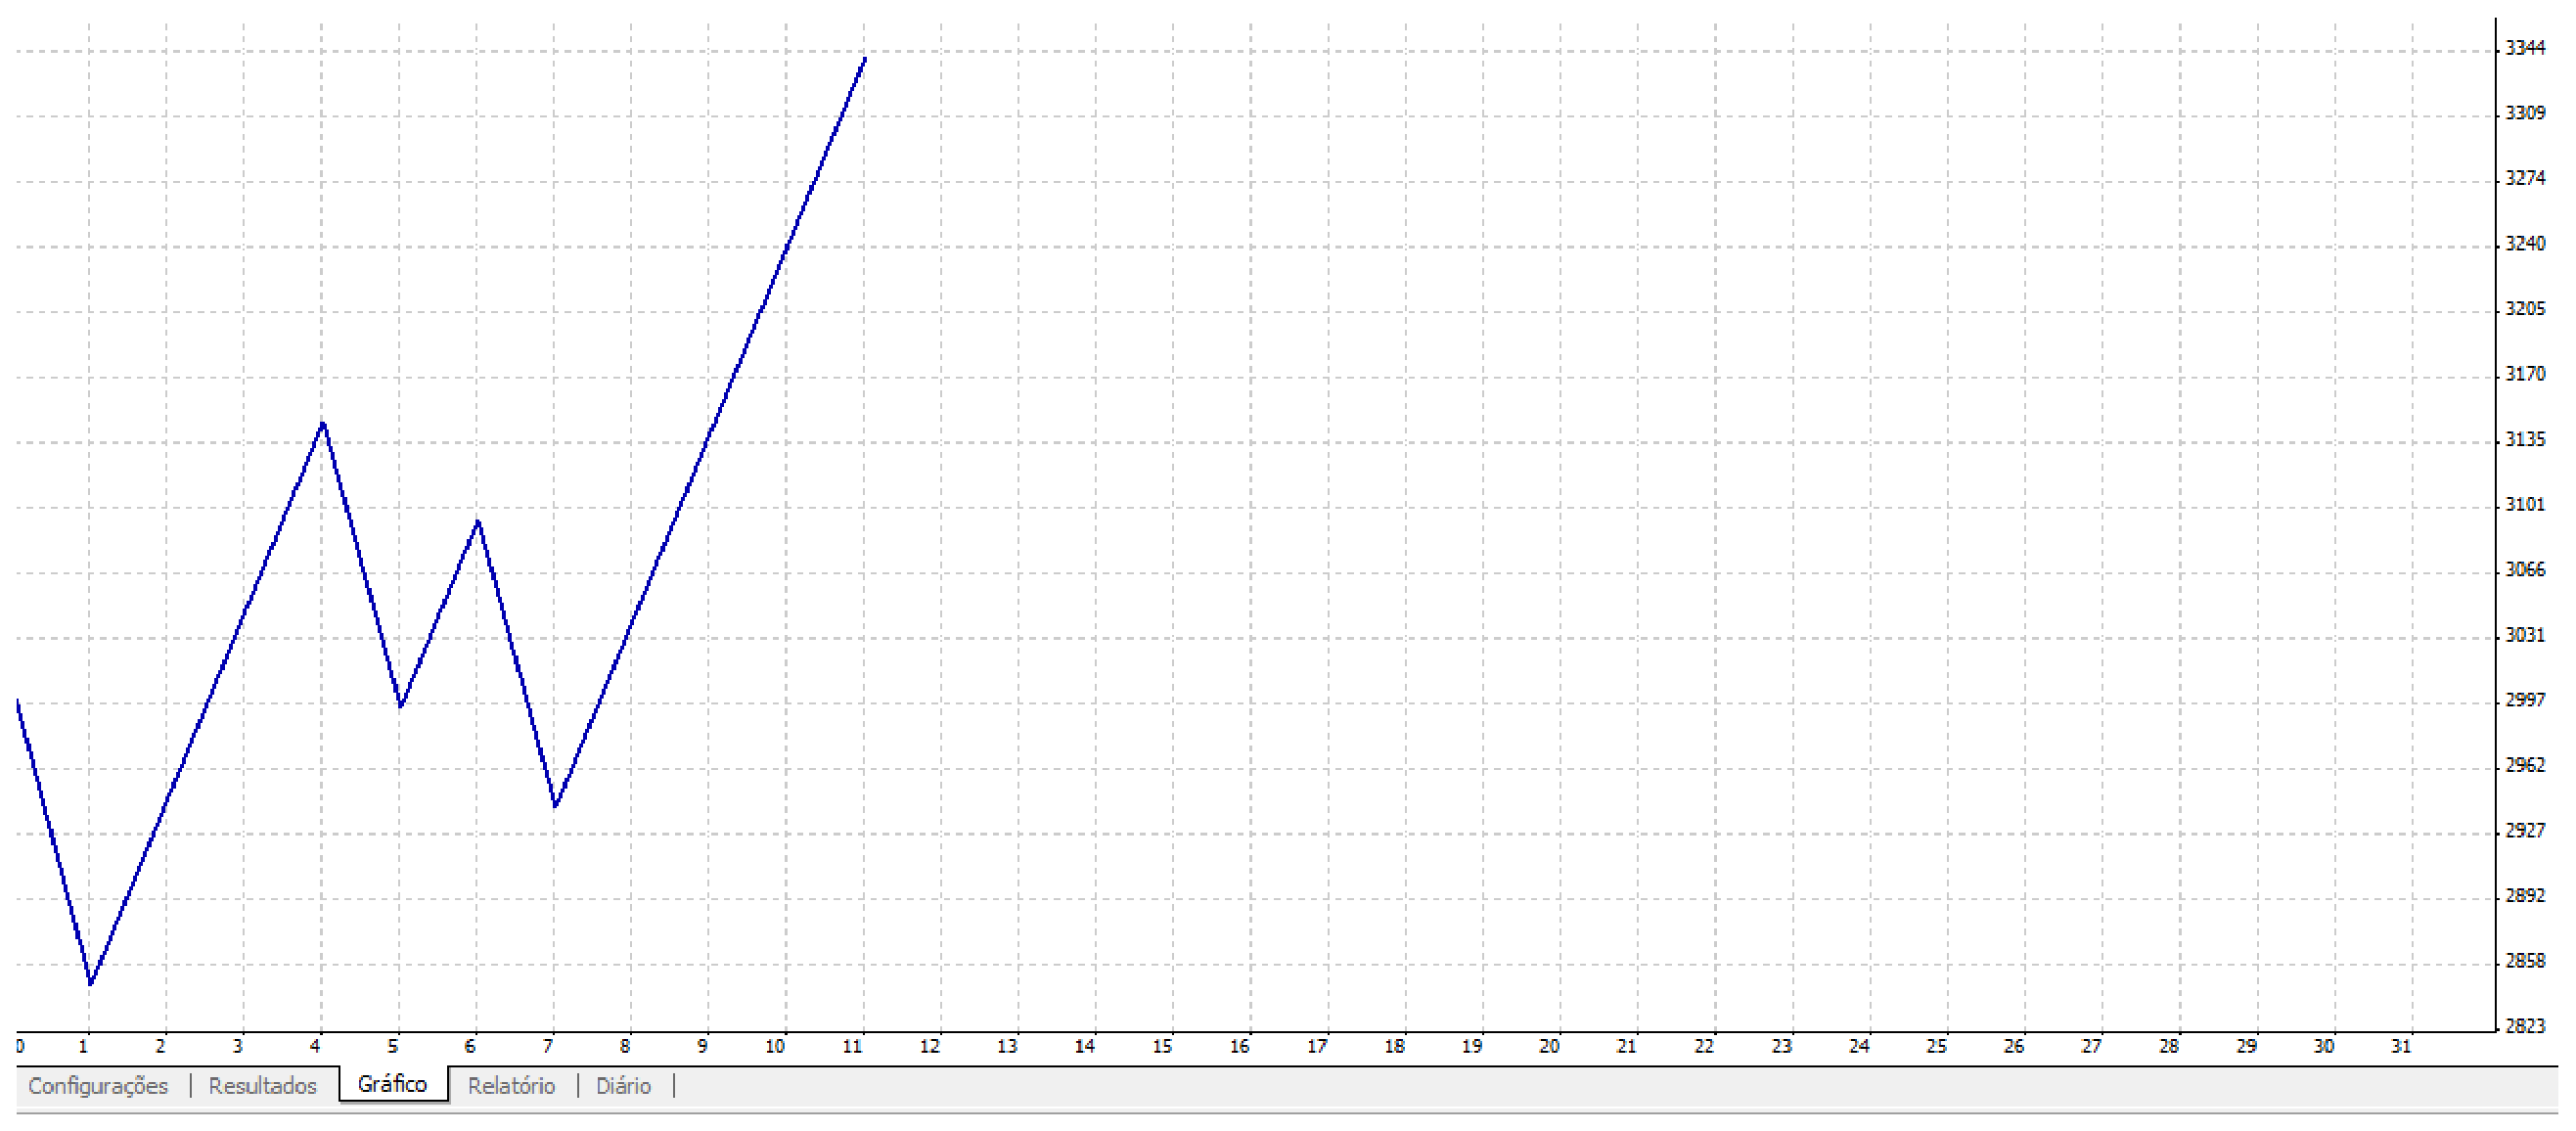
\includegraphics[width=0.9\textwidth]{figuras/protocoloFib4}
\caption{Gráfico gerado pela simulação do expert Fibonacci.mql no período agosto 2013-2014}{Fonte: Autores} 
\label{protocoloFib4}
\end{figure}

\subsection{Simulação do método de Estocástico}

O expert Estocastico.mql obteve o percentual de negociações com lucros de 47.47\% no período agosto 2012-2013. Portanto, o percentual de negociações com perdas foi de 52.53\%. Nesse período, o expert teve um prejuízo de 1110.88 USD.

No período de agosto 2013-2014, o percentual de negociações com lucros foi de 47.70\% (percentual com perdas de 52.30\%)  e obteve-se o prejuízo de 459.17 USD. 
Os relatórios completos das simulações podem ser visualizados nas figuras \ref{protocoloEst} e \ref{protocoloEst2}.

\begin{figure}[htp]
\centering
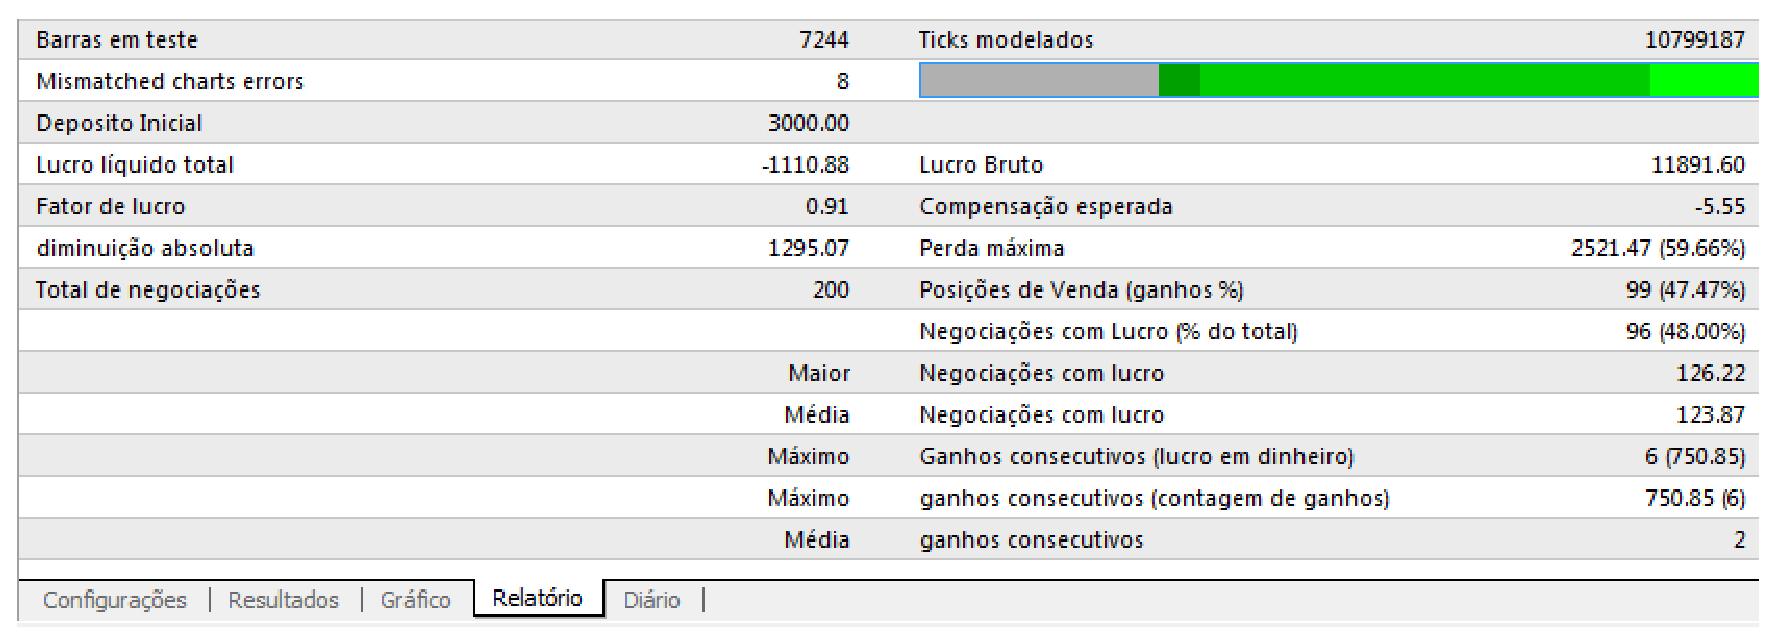
\includegraphics[width=0.9\textwidth]{figuras/protocoloEst}
\caption{Relatório de simulação no período agosto 2012-2013 do expert Estocastico.mql}{Fonte: Autores} 
\label{protocoloEst}
\end{figure}

\begin{figure}[htp]
\centering
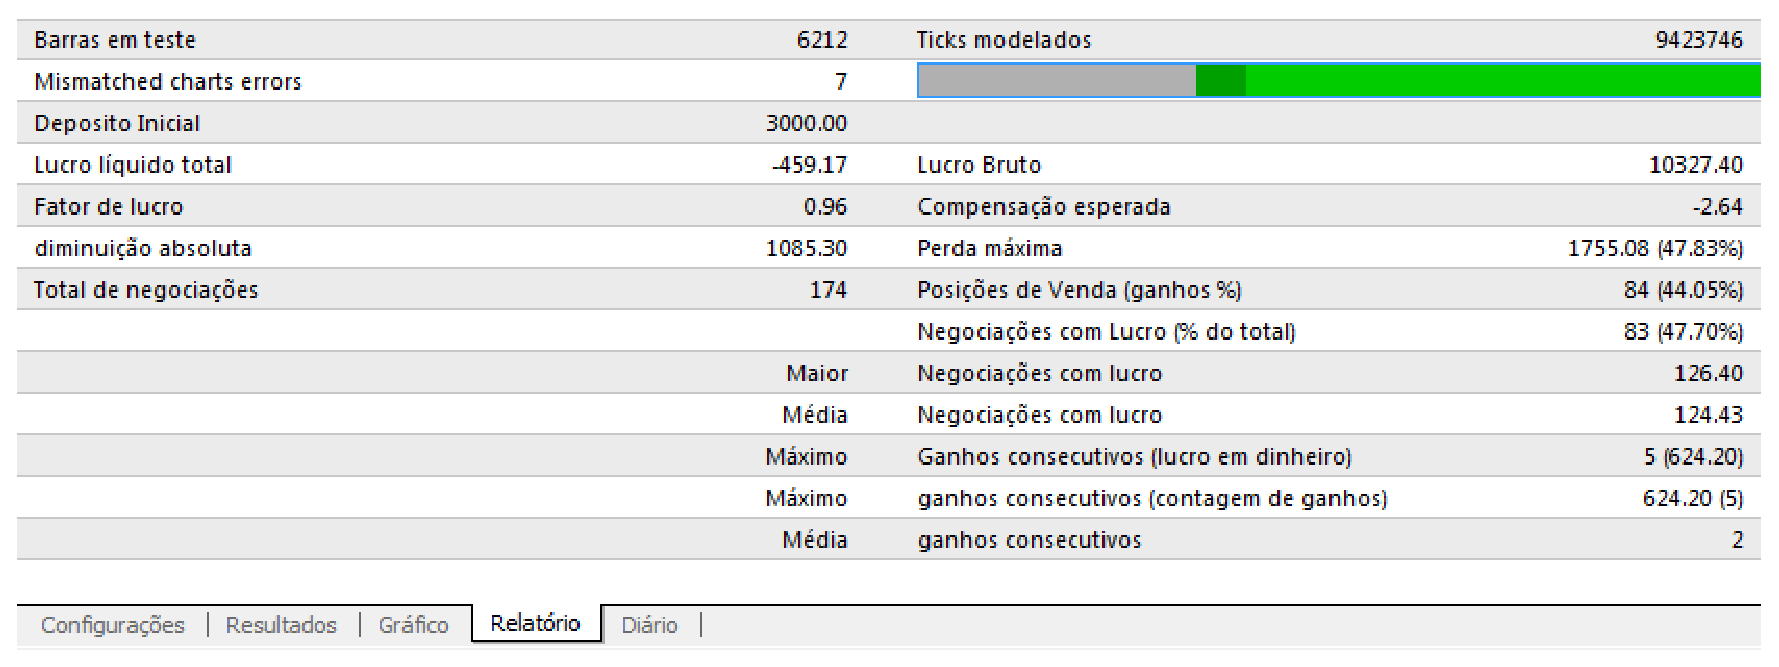
\includegraphics[width=0.9\textwidth]{figuras/protocoloEst2}
\caption{Relatório de simulação no período agosto 2013-2014 do expert Estocastico.mql}{Fonte: Autores} 
\label{protocoloEst2}
\end{figure}

É possível visualizar nos gráficos das simulações, as perdas de capital que o expert Estocastico.mql gerou.

\begin{figure}[htp]
\centering
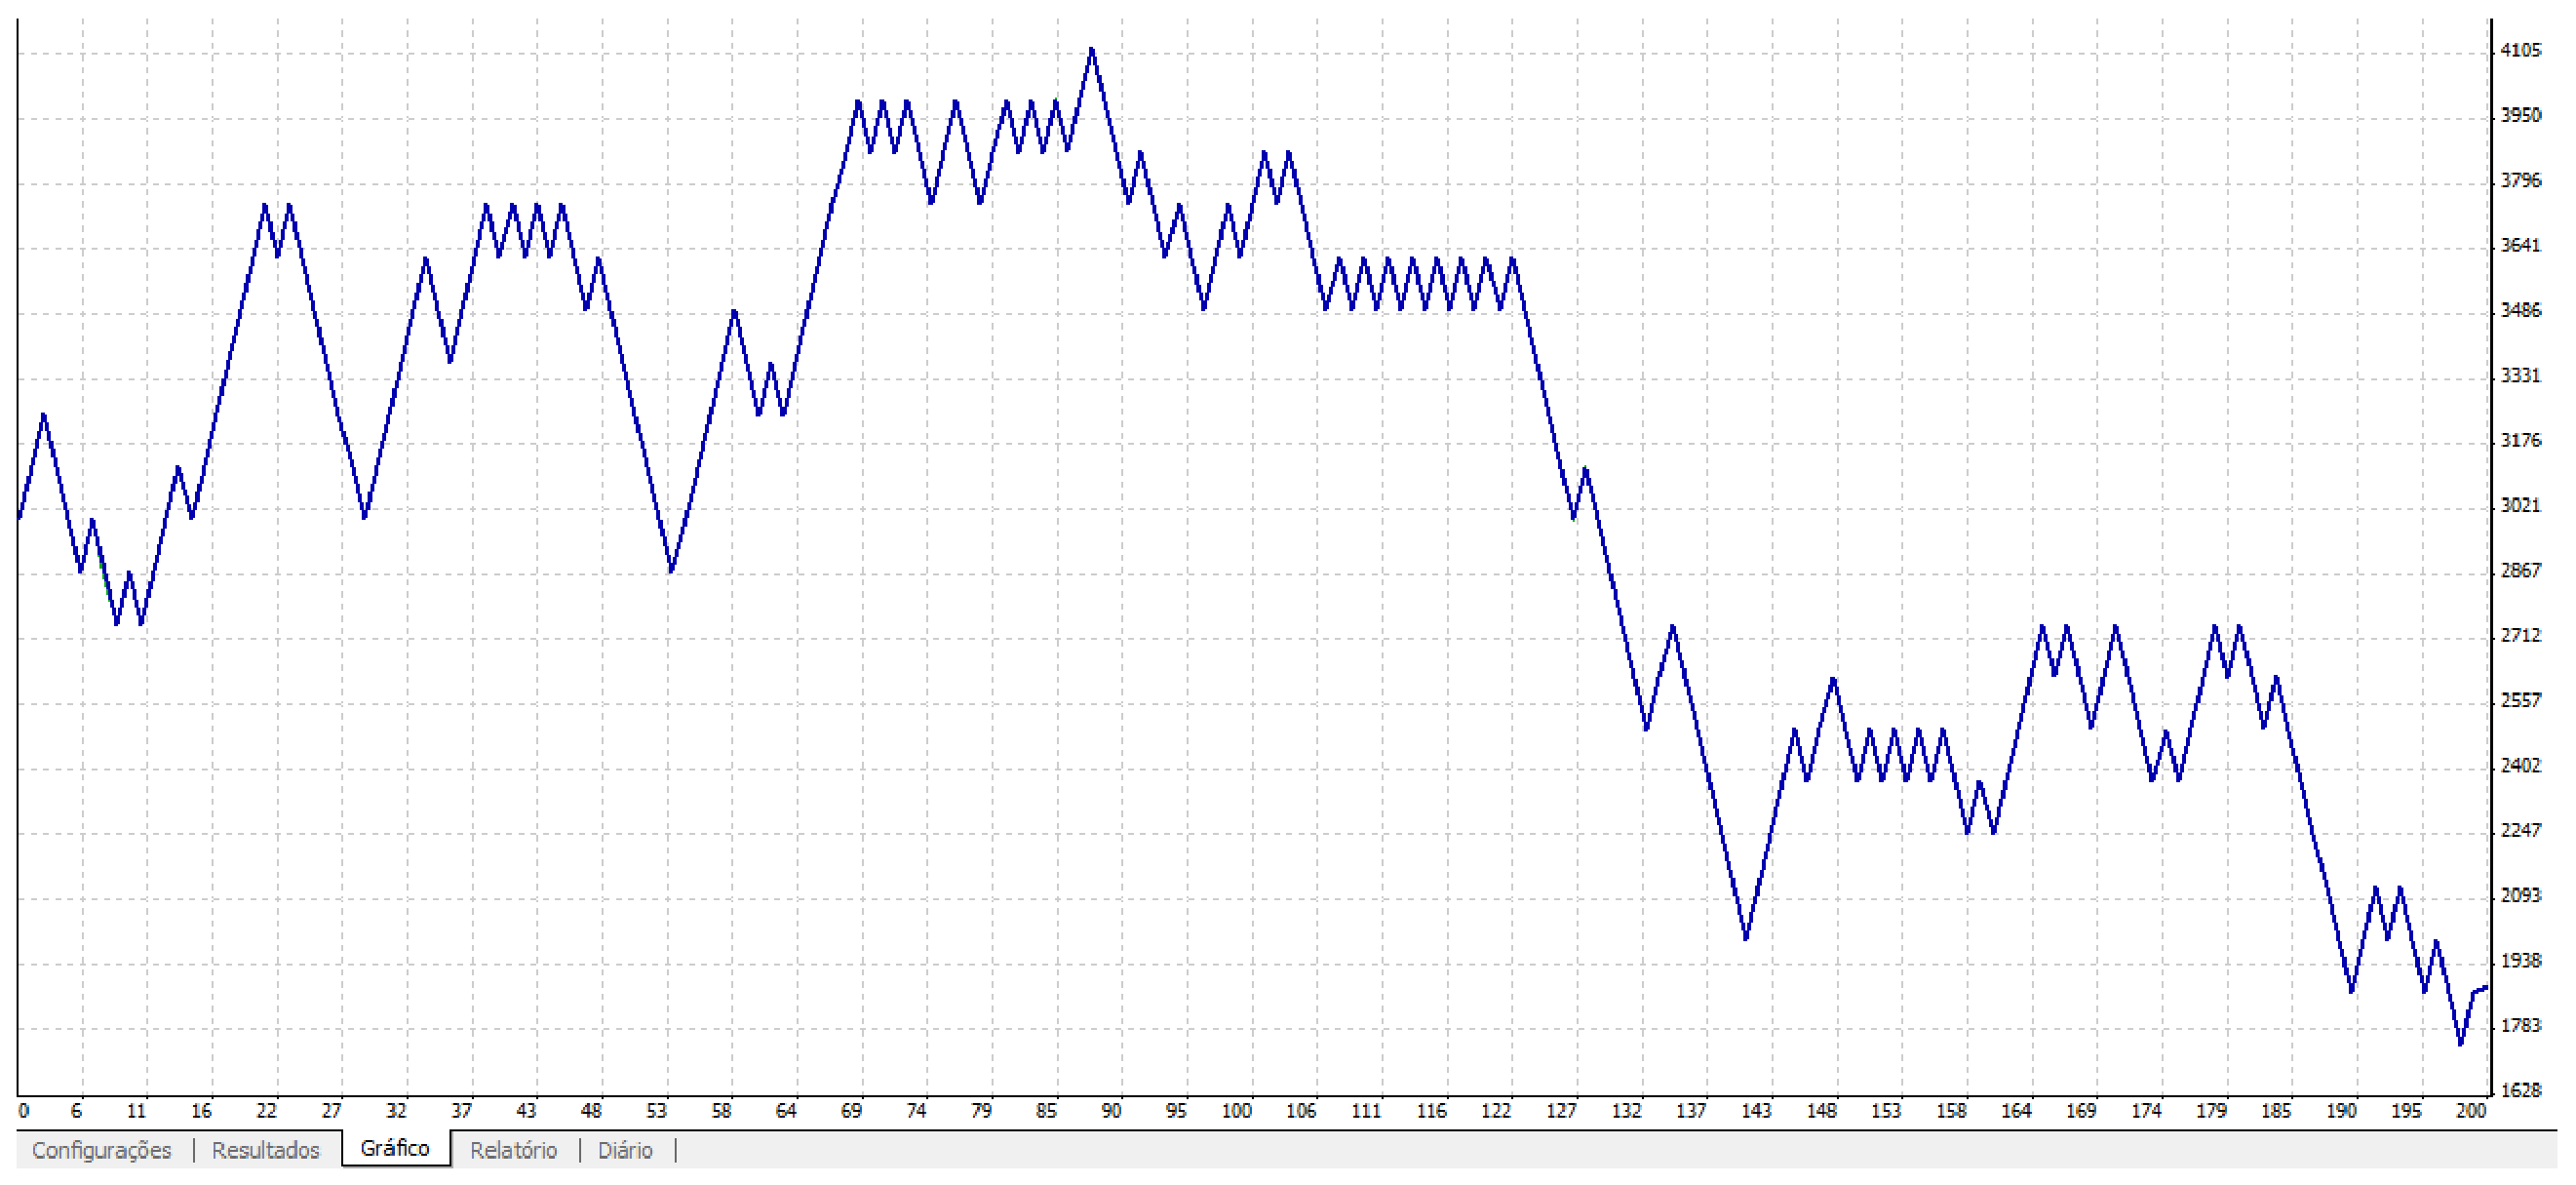
\includegraphics[width=0.9\textwidth]{figuras/protocoloEst3}
\caption{Gráfico gerado pela simulação do expert Estocastico.mql no período agosto 2012-2013}{Fonte: Autores} 
\label{protocoloEst3}
\end{figure}

\begin{figure}[htp]
\centering
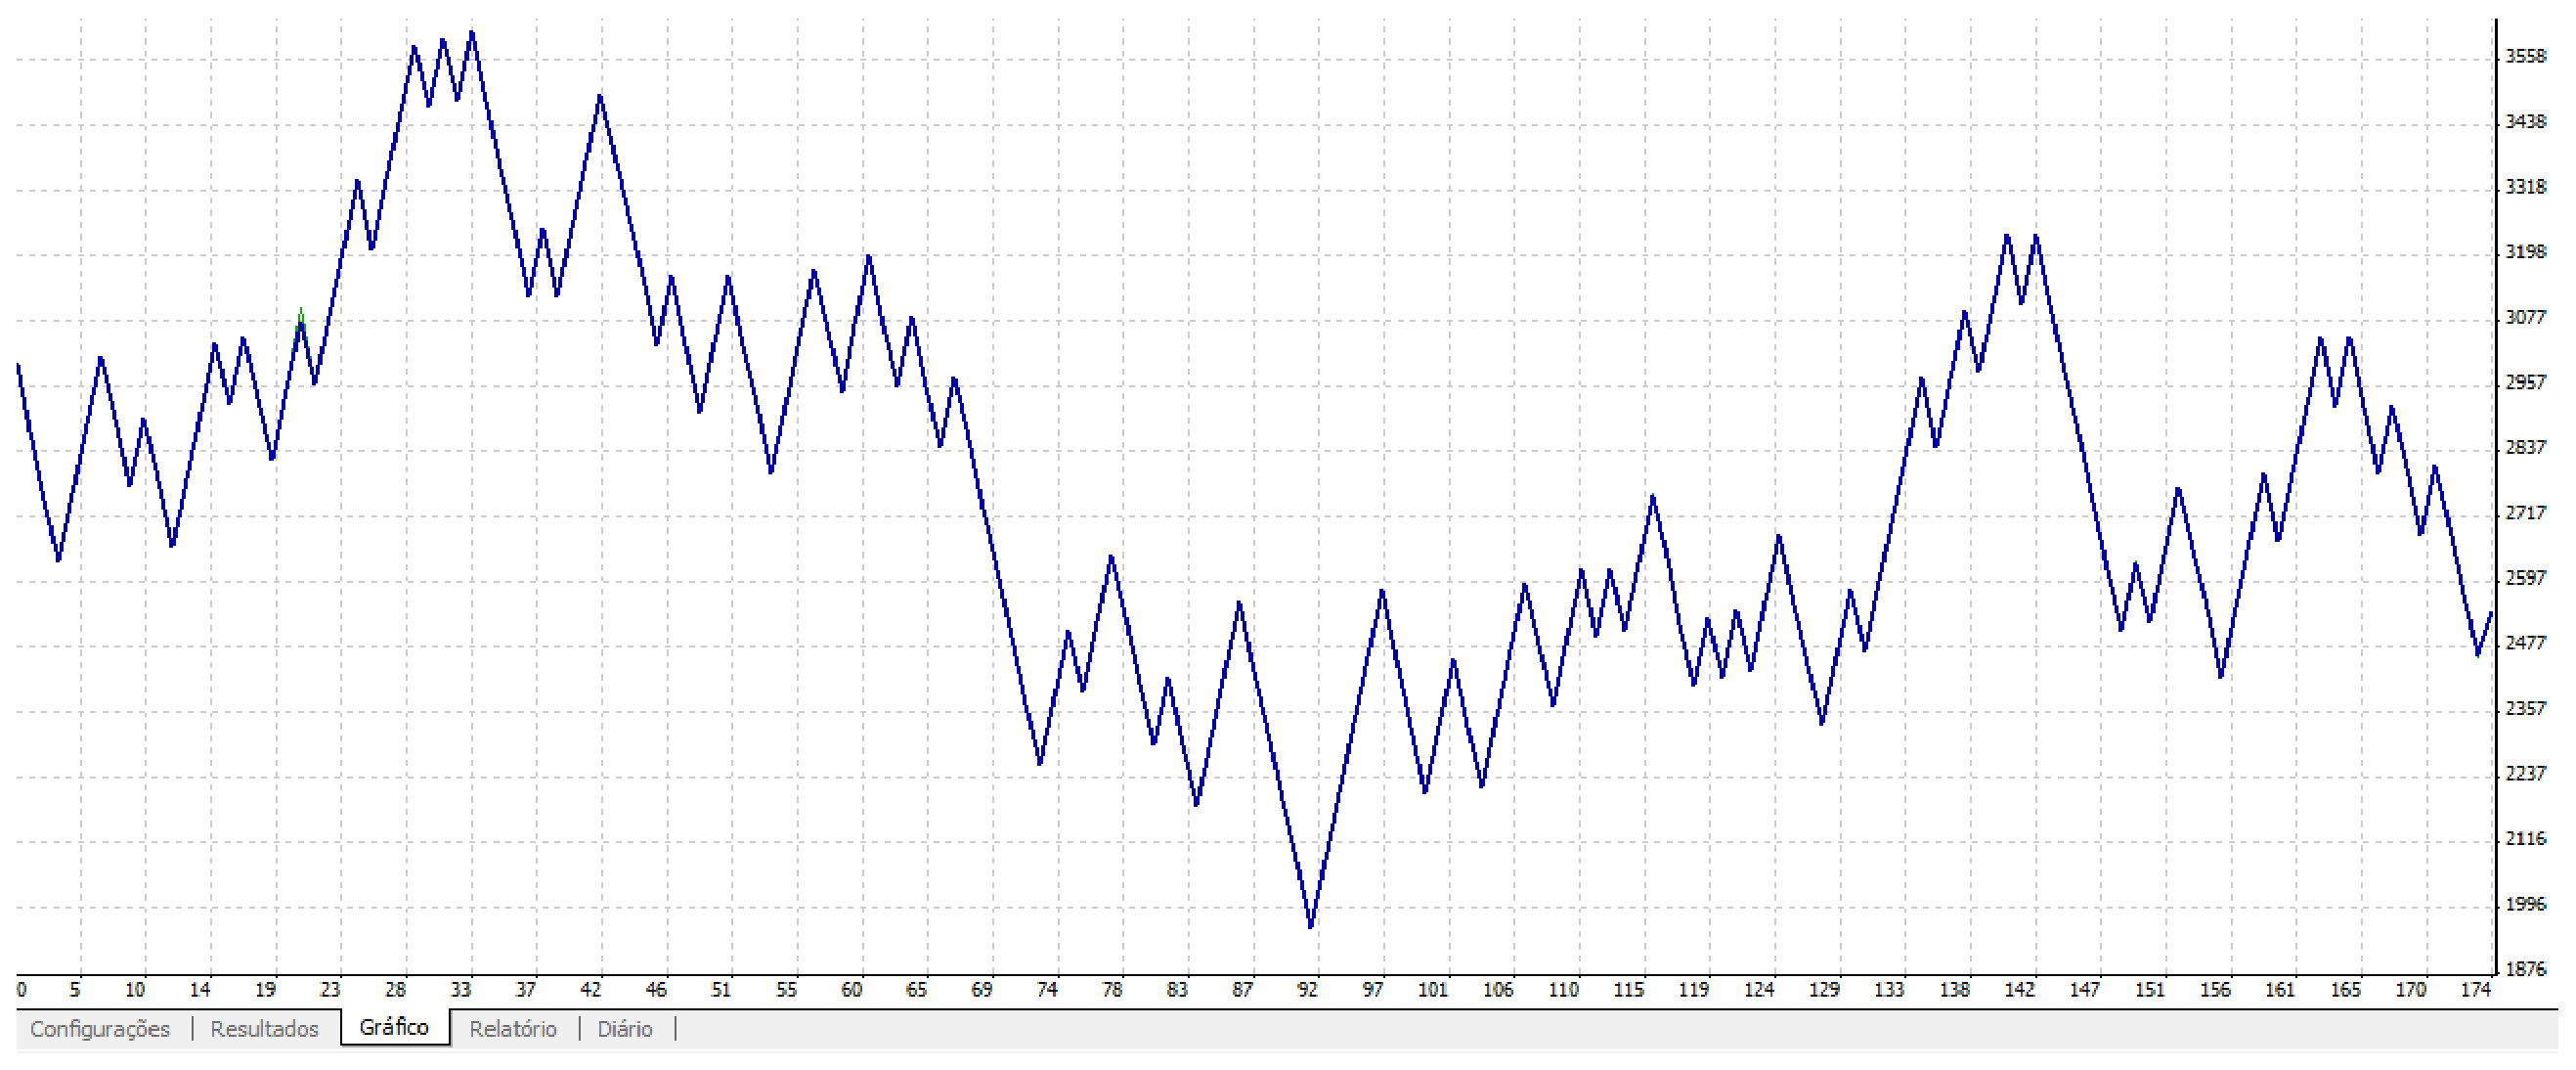
\includegraphics[width=0.9\textwidth]{figuras/protocoloEst4}
\caption{Gráfico gerado pela simulação do expert Estocastico.mql no período agosto 2013-2014}{Fonte: Autores} 
\label{protocoloEst4}
\end{figure}

\subsection{Simulação do método de Média Móvel}

O expert MediaMovel.mql obteve o percentual de negociações com lucros de 43.55\% no período agosto 2012-2013. Portanto, o percentual de negociações com perdas foi de 56.45\%. Nesse período, o expert obteve um prejuízo de 2987.00 USD. 

No período de agosto 2013-2014, o percentual de negociações com lucros foi de 48.48\% e o percentual de negociação com prejuízos foi de 51.82\%.  Foi obtido o prejuízo de 459.17 USD. 

Os relatórios completos das simulações podem ser visualizados nas figuras \ref{protocoloMedia} e \ref{protocoloMedia2}.

\begin{figure}[htp]
\centering
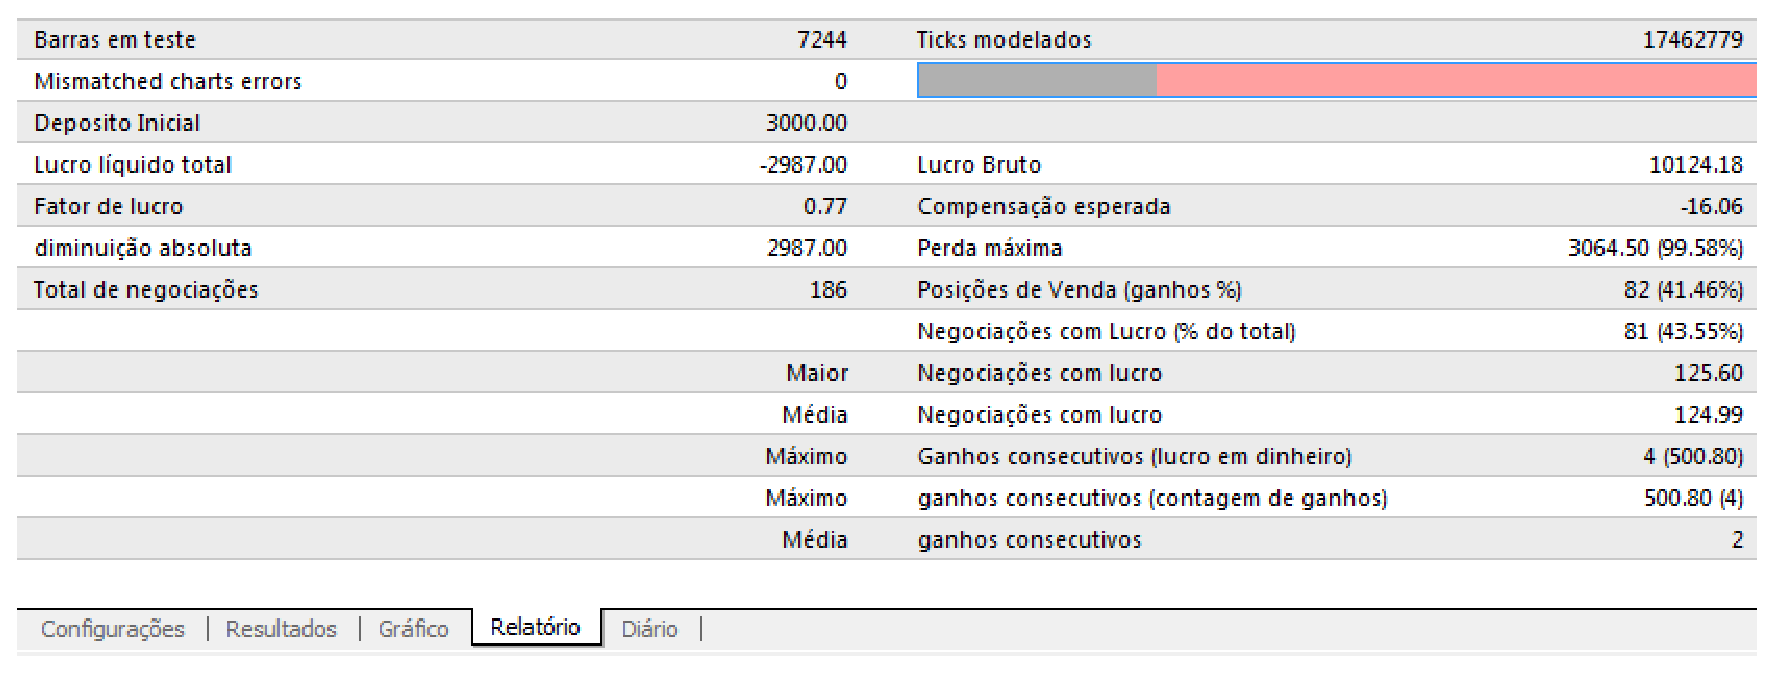
\includegraphics[width=0.9\textwidth]{figuras/protocoloMedia}
\caption{Relatório de simulação no período agosto 2012-2013 do expert MediaMovel.mql}{Fonte: Autores} 
\label{protocoloMedia}
\end{figure}

\begin{figure}[htp]
\centering
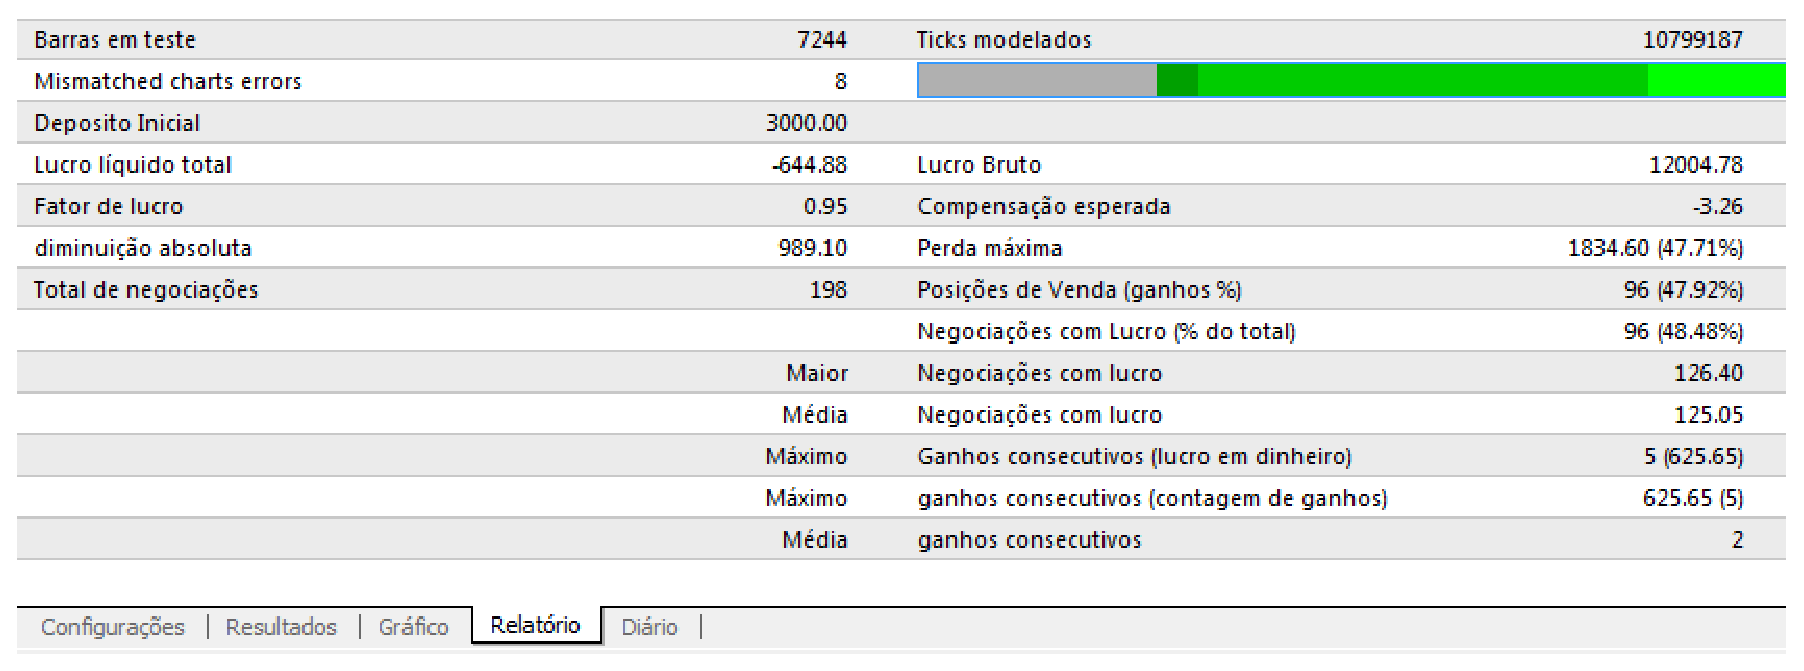
\includegraphics[width=0.9\textwidth]{figuras/protocoloMedia2}
\caption{Relatório de simulação no período agosto 2013-2014 do expert MediaMovel.mql}{Fonte: Autores} 
\label{protocoloMedia2}
\end{figure}

É possível visualizar nos gráficos das simulações, as perdas de capital que o expert MediaMovel.mql gerou.

\begin{figure}[htp]
\centering
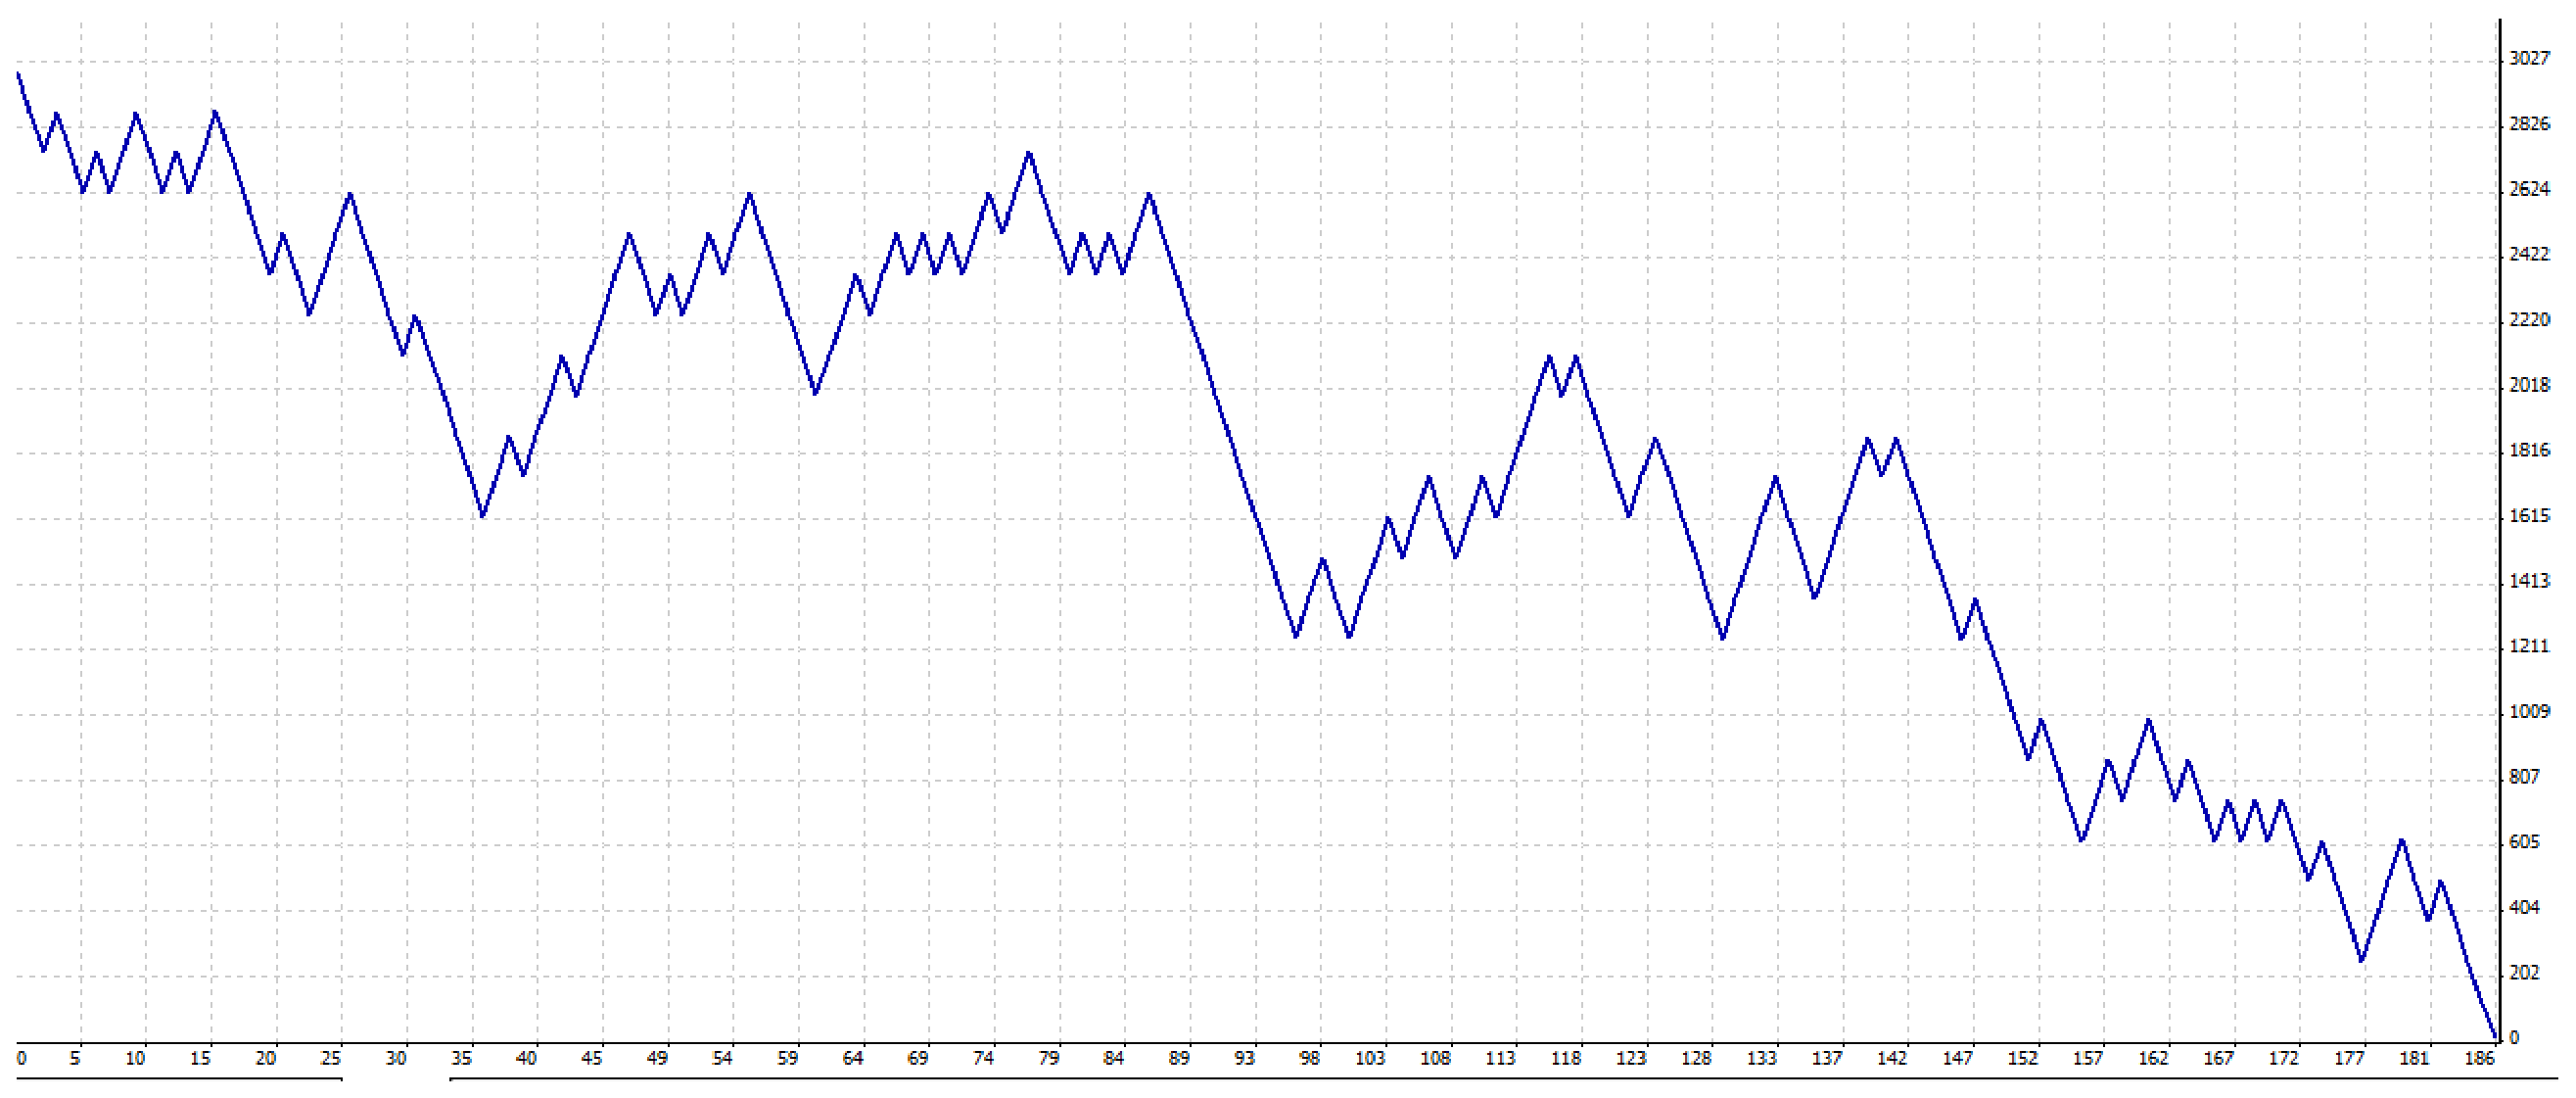
\includegraphics[width=0.9\textwidth]{figuras/protocoloMedia3}
\caption{ Gráfico gerado pela simulação do expert MediaMovel.mql no período agosto 2012-2013}{Fonte: Autores} 
\label{protocoloMedia3}
\end{figure}

\begin{figure}[htp]
\centering
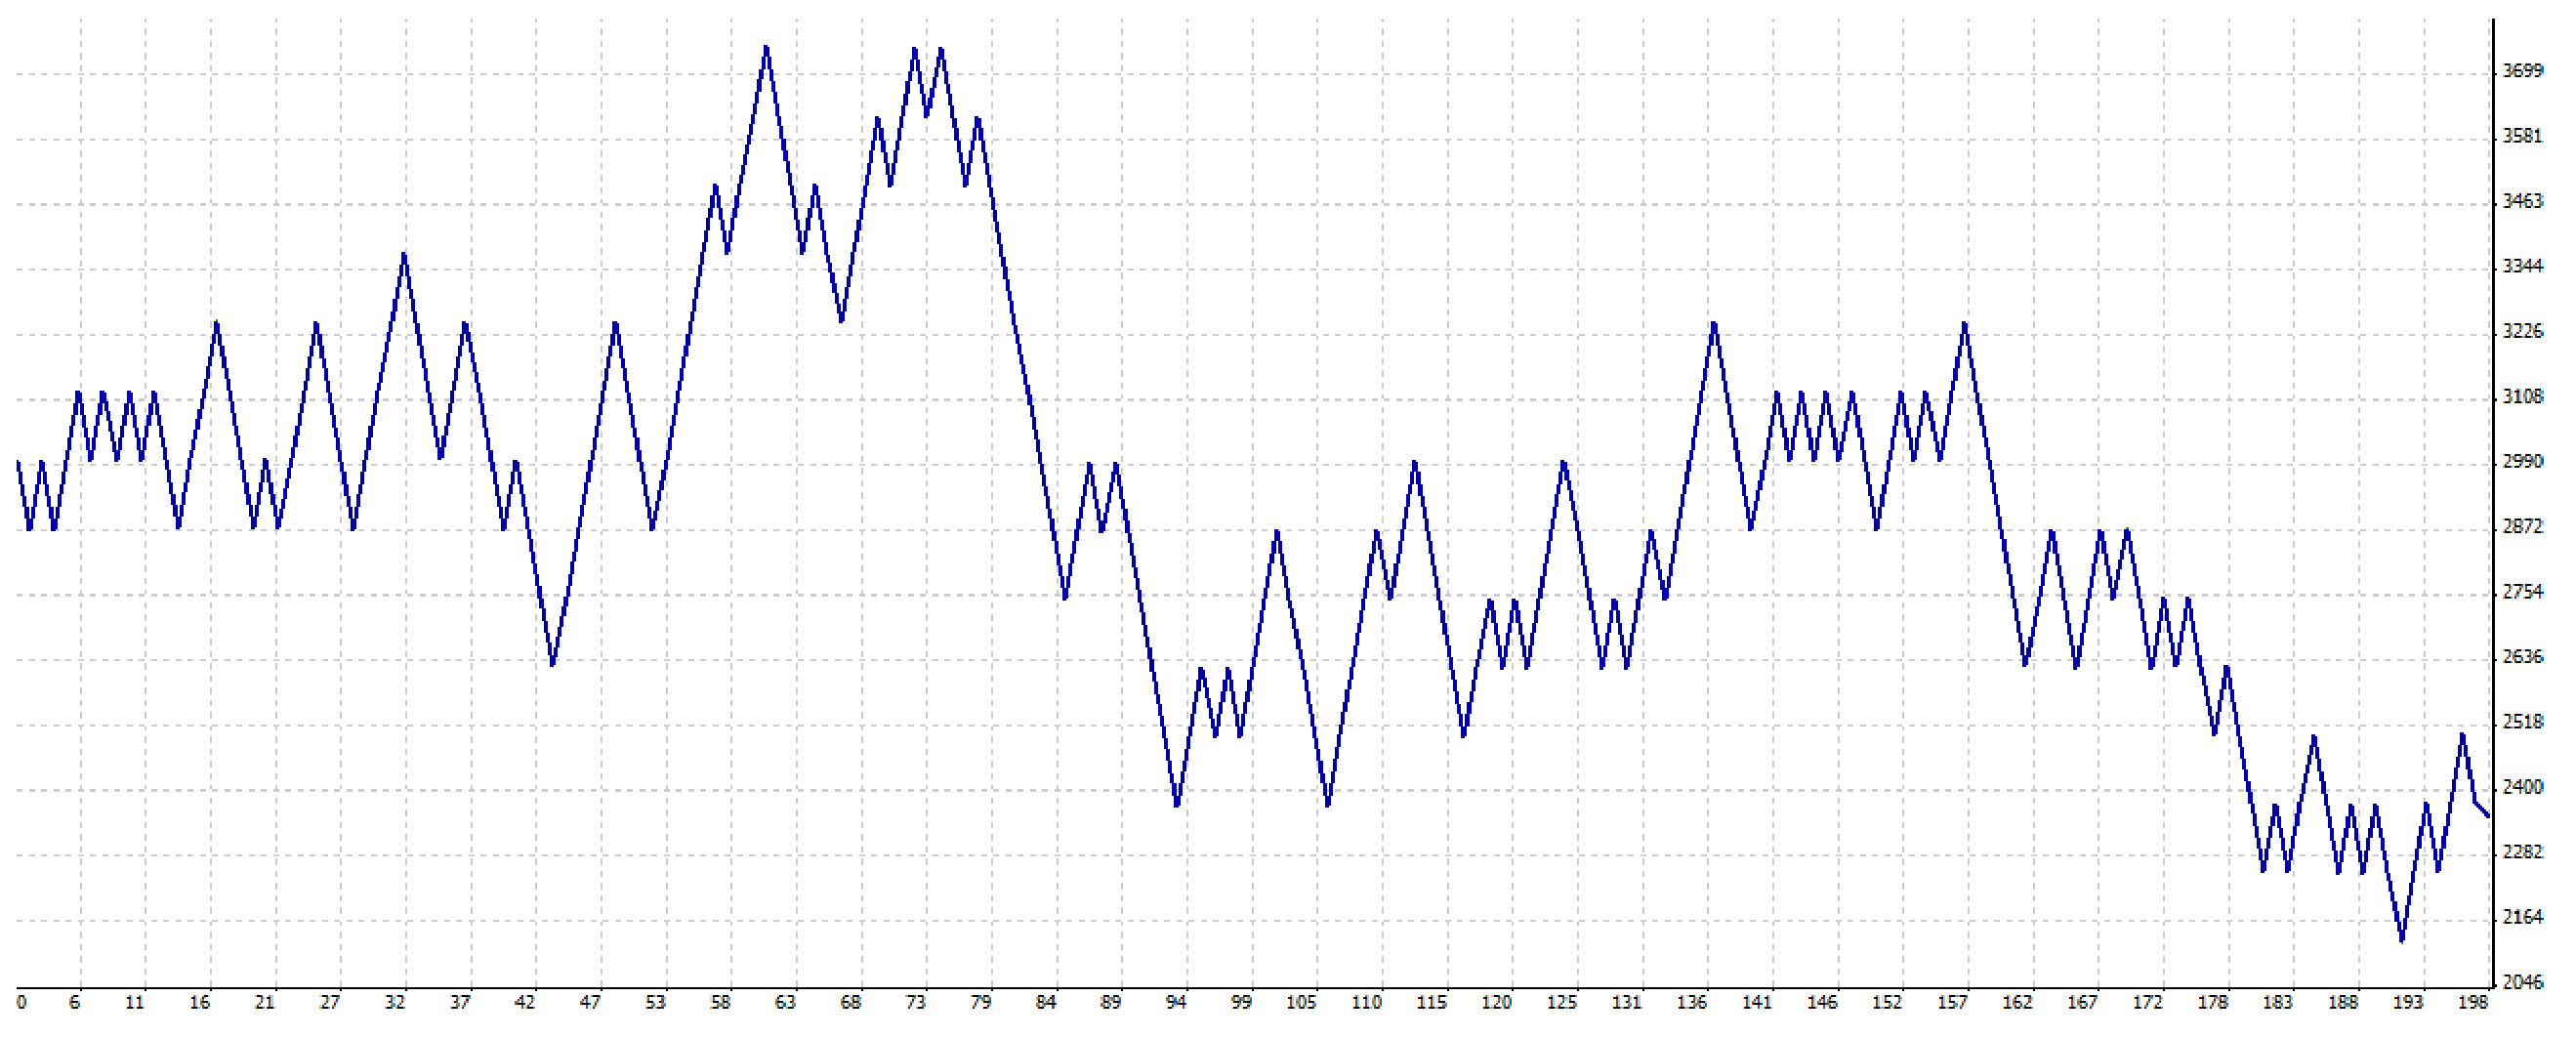
\includegraphics[width=0.9\textwidth]{figuras/protocoloMedia4}
\caption{ Gráfico gerado pela simulação do expert MediaMovel.mql no período agosto 2013-2014}{Fonte: Autores} 
\label{protocoloMedia4}
\end{figure}

\section{Limitações do experimento}

A linguagem MQL4 não possui nenhum suporte para teste unitário. Portanto, os experts programados para este experimento não possuem testes automatizados. 

O simulador MetaTrader possui código fonte fechado. Portanto, não possível realizar nenhum tipo de adaptação do simulador através do código fonte para o experimento.

\section{Definição métodos de operação ferramenta MVC}

Os Métodos Matemáticos de Correlação Linear, Fibonacci e Mínimos Quadrados tiveram êxito nos dois anos de simulação (agosto 2012 a agosto de 2014). Os métodos de Estocástico e Média Móvel tiveram prejuízo nos dois anos de simulação. Portanto, foram escolhidos os métodos de Correlação Linear, Fibonacci e Mínimos Quadrados como métodos de estratégia financeira a serem implementados na ferramenta MVC.
